% THIS IS AN EXAMPLE DOCUMENT FOR VLDB 2012
% based on ACM SIGPROC-SP.TEX VERSION 2.7
% Modified by  Gerald Weber <gerald@cs.auckland.ac.nz>
% Removed the requirement to include *bbl file in here. (AhmetSacan, Sep2012)
% Fixed the equation on page 3 to prevent line overflow. (AhmetSacan, Sep2012)

\documentclass{vldb}
\usepackage{graphicx}
\usepackage{balance}  % for  \balance command ON LAST PAGE  (only there!)
\usepackage[utf8]{inputenc}
\usepackage[english]{babel}
\usepackage{cite}
\usepackage{url}
\usepackage{amsmath}
\usepackage{pifont}
\usepackage{algorithm} 
\usepackage{algpseudocode}

%\usepackage[
%backend=biber,
%style=alphabetic,
%sorting=ynt
%]{babel}
 
% \addbibresource{sample.bib}


\begin{document}

% ****************** TITLE ****************************************

\title{History Reuse K-Means: A new initialization methodology for the classical K-Means for Consistent Speedup}

% possible, but not really needed or used for PVLDB:
%\subtitle{[Extended Abstract]
%\titlenote{A full version of this paper is available as\textit{Author's Guide to Preparing ACM SIG Proceedings Using \LaTeX$2_\epsilon$\ and BibTeX} at \texttt{www.acm.org/eaddress.htm}}}

% ****************** AUTHORS **************************************

% You need the command \numberofauthors to handle the 'placement
% and alignment' of the authors beneath the title.
%
% For aesthetic reasons, we recommend 'three authors at a time'
% i.e. three 'name/affiliation blocks' be placed beneath the title.
%
% NOTE: You are NOT restricted in how many 'rows' of
% "name/affiliations" may appear. We just ask that you restrict
% the number of 'columns' to three.
%
% Because of the available 'opening page real-estate'
% we ask you to refrain from putting more than six authors
% (two rows with three columns) beneath the article title.
% More than six makes the first-page appear very cluttered indeed.
%
% Use the \alignauthor commands to handle the names
% and affiliations for an 'aesthetic maximum' of six authors.
% Add names, affiliations, addresses for
% the seventh etc. author(s) as the argument for the
% \additionalauthors command.
% These 'additional authors' will be output/set for you
% without further effort on your part as the last section in
% the body of your article BEFORE References or any Appendices.

\numberofauthors{2} %  in this sample file, there are a *total*
% of EIGHT authors. SIX appear on the 'first-page' (for formatting
% reasons) and the remaining two appear in the \additionalauthors section.

\author{
% You can go ahead and credit any number of authors here,
% e.g. one 'row of three' or two rows (consisting of one row of three
% and a second row of one, two or three).
%
% The command \alignauthor (no curly braces needed) should
% precede each author name, affiliation/snail-mail address and
% e-mail address. Additionally, tag each line of
% affiliation/address with \affaddr, and tag the
% e-mail address with \email.
%
% 1st. author
\alignauthor
Shanil Puri
       \affaddr{Dept. of Computer Science}\\
       \affaddr{North Carolina State University}\\
       \affaddr{890 Oval Dr, Raleigh}\\
       \affaddr{North Carolina, USA}\\
       \email{spuri3@ncsu.edu}
% 2nd. author
\alignauthor
Xipeng Shen
       \affaddr{Dept. of Computer Science}\\
       \affaddr{North Carolina State University}\\
       \affaddr{890 Oval Dr, Raleigh}\\
       \affaddr{North Carolina, USA}\\
       \email{xshen5@ncsu.edu}
}
% There's nothing stopping you putting the seventh, eighth, etc.
% author on the opening page (as the 'third row') but we ask,
% for aesthetic reasons that you place these 'additional authors'
% in the \additional authors block, viz.
% Just remember to make sure that the TOTAL number of authors
% is the number that will appear on the first page PLUS the
% number that will appear in the \additionalauthors section.


\maketitle

\begin{abstract}
In this data explosion era, there are myriad programs that are executed repeatedly on large sets of data, consuming high amounts of energy and resources. Critical process reused on different data sets will no doubt help reduce the time and computations.

This thesis explores how Computation Reuse can be implemented for augmenting the performance of some time consuming data analytics algorithms. Specifically, we developed a general framework for efficiently finding similar datasets and effectively reusing history. We demonstrated the large benefits (up to 20X in average case and upto 200X in best case) on K-means and SGD-based SVM algorithm.
\end{abstract}

%################### START OF INTRODUCTION ###################
\section{Introduction}
In this data explosion era, there are myriad programs that are executed repeatedly on large sets of data, consuming high amounts of energy and resources. Critical process reused on different data sets will no doubt help reduce the time and computations. In this work we will introduce a new probabilistic model of measuring data similarities. Based on these data similarities we will show how critical computations may be reused across data sets, saving energy and improving performance.

Our work will introduce a general architecture for comparing two or more data sets and get a probabilistic measure of similarity. We reason that if two data sets are similar, computation reuse from previous iteration of an algorithm for the similar data set will provide a good speed up in the execution of the algorithm for the current data set.
We first define the architecture to compute the above-mentioned metric of similarity and then proceed to validate our above-mentioned stipulation for the K-Means and the SGD based SVM algorithms.

In these explorations, we found challenges in 4 aspects: \textbf{data features, similarity definition, scalability,} and \textbf{reuse}. Data features, is the description of data sets. Similarity definition (distance between two data sets) is the metric we use to describe similarity between data sets. Data feature and distance definition are used together for reuse instance selection from a program specific database. The selection of history record is the most essential part of computation reuse.

Since the method used to calculate distances between two data sets, should also be defined based on data features, the problem becomes even more complex. Scalability issues are related with number of instances in database, size of the target data set, and dimension of data-set. Goal of computation reuse is to save computation time and energy. In order to select a suitable history record, some extra computation is inevitably introduced. The dilemma is the trade-off between the amount of computation reuse and the introduced overhead. 

Reuse, thus is the process to decide what history information the program should reuse and how to reuse the pre-computed information.
In this study we introduce the concept of Historical Computation reuse. This is an Intuitive Idea whose exploration for the family of algorithms mentioned above is spotted at best.

\textbf{\textit{Computation Reuse}} is the process of deciding what history information the program should reuse and how to best reuse the pre-computed information.
While the idea is simple and intuitive in nature, it promises big gains if correctly implemented with a wide variety of uses.
In this study we give an empirical study, showing that effectively computation reuse could enhance program performance.
Although, the idea of computation reuse is simple, there are many difficulties need to be solved to achieve efficient and effective reuse. 
In our explorations, we found out challenges in 4 aspects: data feature abstraction, similarity definition, scalability, and reuse. 
\textit{Data Features}, is the description of data sets. The major challenged we faced in \textit{Data Feature Abstraction} was to reduce dimensionality (for the sake of optimization), while preserving the integrity of data.
\textit{Similarity definition} (distance between two data-sets) is the way we would like to describe similarity between two data set. The challenge was to come up with a meaningful metric to give an accurate prediction of suitability for reuse. 
We used \textit{Data feature abstraction} and \textit{Similarity definition} together for reuse instance selection from a program specific database. The selection of history data set is the most essential part of computation reuse because different data sets will lead to dramatically different computation times. Because the most important properties of the input data may vary on different programs, it is difficult to decide a universal data feature and data distance definition. Since the method used to calculate distances between two data sets descriptions also should be defined based on the data features, the problem becomes even more complicated. 
\textit{Scalability} issues are related with number of data set instances in database, size of the target data set, and its dimensionality. Goal of computation reuse is to save computation time and energy. In order to select a suitable history record, some extra computation is inevitably introduced into the computation. The dilemma is the tradeoff between the amount of computation reuse and the introduced overhead. For example, increase the number of instances in database will increase the probability of finding a good history record. However, it will also increase the introduced selection overhead. The size of target data set and the dimensionality of would also produce similar issues.
\textit{Reuse} is the process of deciding what history information the program should reuse and how to reuse this pre-computed information. Challenges in this field are mainly caused by the differences among programs and algorithms. For a specific program or algorithm, it might be a trivial solution while for another selecting historical data may be a complex problem. Our approach of building a general framework to work as a plug and play device makes the process even more complicated. 
In this work, we investigate multiple solutions to address each of the challenges, and come up a framework, which we will apply to two of commonly used algorithms, namely: \textbf{\textit{K-Means(Lloyd’s Clustering algorithm)}} and the \textbf{\textit{Stochastic Gradient Decent based Support Vector Machine}} for our explorations and providing proof of effectiveness of History Reuse and to validate the efficiency and the effectiveness of our algorithm.
The paper is organized in the following sections: Section \textit{\ref{chap-two}} gives motivation, background and definitions of terms we use in this paper. Section \textit{\ref{chap-three}} will give formal definition to the challenges we faced and our approach for coming to a successful conclusion. Section \textit{\ref{chap-four}} will formalize the framework and give the formal algorithm for our architecture. We will also discuss the other approaches we used to come to our conclusions and give reasons for their failures. We present the evaluations for our algorithm in Section \textit{\ref{chap-five}}.Future work is discussed in Section \textit{\ref{chap-six}}, while Section \textit{\ref{chap-seven}} provides conclusion derived from our explorations.

%################### END OF INTRODUCTION ###################


%################ MOTIVATION AND BACKGROUND ###################
\section{Motivation and Background}
\label{chap-two}
\subsection{Motivation}
Computation reuse across executions benefits programs with long computation time most, especially converging algorithms that require multiple iterations to compute desired results. This class of problems as such has no generic polynomial time algorithms, thus making history reuse for predictive initialization a good candidate for optimization. Another benefit may be improved accuracy. Through appropriate history result reuse, numbers of iterations of computations could be saved while the accuracy gets improved. The key point of computation reuse on different data is finding suitable history information to reuse. Thus, the above stated problem essentially boils down to introducing a probabilistic method of calculating data set similarities quickly and accurately. With databases containing a number of instances, data set features is a key component of each instance, and history computation result of the program on this data set is the value. Then, through computing distance from current data set to each instance, our framework could select the instance, which has the highest probability to provide most effective computation reuse.
Optimization of converging Algorithms such as K-means clustering and SGD based SVM are highly beneficial. Algorithms of this category are used frequently and have a multitude of applications in real world machine learning and big data processing.  Some of the motivations for this work may be listed as follows:
\begin{itemize}
	\item \textit{Frequently Used:} These algorithms are used frequently to tackle real world problems and thus even small improvements can have a significant impact.
	\item \textit{Wide Area of Application} These algorithms also have wide areas of real world application ranging from machine learning to big data problems.
	\item \textit{Prime Candidates:} These algorithms are ideal suited for such optimizations, as their speed of convergence and accuracy is directly dependent on the starting points for the algorithm and thus can be used as proof for the benefits of history reuse easily.
\end{itemize}
\subsection{Background and Related Work}
For most part of the generation and the testing of our \textit{History Reuse architecture} we use the classical \textit{K-Means algorithm (Lloyd's Algorithm)}\cite{kmeans_orig} . We then test the architecture with the \textit{Stochastic Gradient Decent based Simple Vector Machines}\cite{sgd_svm} to prove the global viability of our algorithm.
The classic K-Means algorithm (Lloyd’s algorithm) consists of two steps. For an input of 'n' data points of 'd' dimensions and 'k' initial cluster centers, the assignment step assigns each point to its closest cluster, and the update step updates each of the k cluster centers with the centroid of the points assigned to that cluster. The algorithm repeats until all the cluster centers remain unchanged in a single iteration.
Because of its simplicity and general applicability, the algorithm is one of the most widely used clustering algorithms in practice, and is identified as one of the top 10 data mining algorithms (Wu et al., 2008). However, when n , k, or d is large, the algorithm runs slow due to its linear dependence on n, k, and d. There have been a number of efforts trying to improve its speed. Some try to come up with better initial centers (e.g. K-Means{++} \cite{kmeans++} or parallel implementations \cite{kmens_parellel}. This thesis will look to present more on this approach by exploring an avenue not much pursued before, namely historical data set cluster center reuse for K-Means Initialization. 
Prior efforts in this direction include: K-Means{++}(Arthur and Vassilvitskii, 2007; Bahmani et al., 2012), K-Means Initialization Methods for Improving Clustering by Simulated Annealing (Gabriela Trazzi Perim et al. 2008), an optimized initialization center K-Means clustering algorithm based on density (Xiaofeng Zhou et al. 2015). These prior methods, while having made a significant contribution, have failed to replace the Lloyd`s algorithm which still remains the dominant choice in practice exemplified by the implementations in popular libraries, such as GraphLab (Low et al.), OpenCV, ml-pack (Curtin et al. 2013) and so on.
Previous implementations that have tried to optimize the selection of the initial centroids based only on the current data set. For instance, the original K-Means Algorithm (Lloyd’s algorithm) chooses \textit{k} cluster centers randomly from the points available in the current data set. The K-Means{++} \cite{kmeans++} further optimizes this by taking steps to increase probability of getting good starting points by first choosing a random centroid and then proceeding to choose the furthest possible centroid from last chosen centroid iteratively, doing this for each centroid computation. The approximation method for initialization \cite{approx_meth}, aims to approximate the selection of centroid, but this approach produces clustering results different from the results of the standard K-Means. The above algorithms as can be seen work only on the current data set at hand. No prior work has directly tried to systematically exploit historical data for computation, which forms the basis of this thesis.
This work will introduce and formalize the History Reuse Architecture. We will then use \textit{History Reuse} to introduce a new Initialization methodology for the K-Means algorithm: "Historical dataset center reuse for K means initialization", an enhanced K means implementation which aims to optimize the K means algorithm by aiming to choose the best possible starting points for the K-Means\cite{kmeans_orig} for faster convergence. Since the only modification that are being made are in the initialization step of the algorithm it stands to reason that the algorithm would continue to uphold the same standards as the standard K-Means algorithm. We will also use our History Reuse Architecture and test it for SGD based SVM\cite{sgd_svm} to prove the global application of our generic architecture.

While history reuse has been prevalent and an area of great exploration as of late, this approach of utilizing offline computed training data for History Reuse is unique and as such has not been explored. History Reuse though has been seen in myriad other works including Yinyang K-Means \cite{yinyang_kmeans} where in pre-computed geometrical information for distances for points from centroids is stored and reused in the multiple iterations of the algorithm in a single run. It makes use of this information for both initialization and re-labeling of points by reusing distance computation information. Similarly, the K-means optimized by Elkan \cite{Elkan03usingthe} and by Drake and Hamerly\cite{drake} also computes the triangular inequality and uses it to optimize run time by minimizing computations of distance per iteration by reusing the precalculated distance bounds with changes in the limit of the distances maintained in history on a per iteration basis.

Compiler studies have also had a lot of work done in the area of history reuse for code optimization such as the "Automated Locality Optimization Based on the Reuse Distance of String Operations" \cite{auto_cache_opt} which aims to use call context on Cache hits for optimal use of L2/L3 caches. These and other works\cite{value_reuse_extended}\cite{load_reuse_proceeding}\cite{load_reuse_proceeding_article}\cite{locality_block_reuse} have often used history reuse in the optimization at the micro or program level. 

Some of the other specific works in optimizing the K-Means algorithm \cite{kmeans_orig}, which is also a product of this thesis, have used myriad approaches for optimizing the K-Means algorithm. Some optimizations use approximation methodologies (\cite{Czumaj}; \cite{Sculley}; \cite{4270197}; \cite{Guha:1998:CEC:276305.276312}; \cite{Zeng:2012:FAK:2354409.2354758}) while other try to speed up K-Means inherently, while trying to maintain the semantics of the original algorithm. An example of the latter is to speed up the algorithm using KD-Trees \cite{Pelleg:1999:AEK:312129.312248}\cite{Kanungo:2002:EKC:628329.628801} which show promise for smaller cluster sizes but do not perform as well for larger cluster sizes.

With our proposed solution we extend this approach to a macro level choosing to look at the problem at the data level as compared to the optimizations done at program level. Since our approach is program independent to a large extent, our algorithm will work as a generic framework for all data related optimizations and can be directly combined with any program level optimization to achieve further speedups. For instance, we may use our approach in conjunction with the above mentioned Yinyang K-Means implementation to optimize the initialization as well iteration time for a single run of the algorithm. This way we stand to gain the best of both worlds by combining both program level and data level optimizations.


\subsection{Important Terminology}
For the propose of our discussion we assume data to be represented in a \textit{2-D matrix} where in each \textit{row} represents a \textit{single point} in a data set while the \textit{columns} are used to represent the \textit{feature set} of each point.
The following are important terms for this work and are used through out the later chapters:
\begin{itemize}
	\item \textbf{Data Source}: These are the actual sources of Data Set repositories from which we source our data for testing purposes.
	\item \textbf{Data Set}: Data on which the actual algorithm is run after dividing the data from the \textit{Data Source}. Each \textit{Data Set} is built up of multiple \textit{Data Items or Data Points}.
	\begin{itemize}
		\item \textit{Current Data Set:} Represents the data set on which the current iteration of the algorithm is to be run.
		\item \textit{Historic Data Set:} Data Set present in the History Data Base for which results have been computed in previous iterations of the algorithm, making the data set one of the viable candidates for \textit{History Reuse} for \textit{Current Data Set.}
		\item \textit{Data Item / Data Point:} Single row in Data set. Represents a single data point in the larger \textit{Data Set}.
		\item \textit{Dimensionality(d):} Number of columns used to represent a single \textit{Data Item.}
	\end{itemize}
	\item \textbf{History Data Base:} Data base for storing all data sets that may be candidates for \textit{History Reuse} for \textit{current data set} and for which final results have been calculated in previous iterations of the algorithm.
	\item \textbf{Cluster Count (k):} The total number of cluster in which the \textit{Data Set} is to be clustered when using the \textit{K-Means Algorithm}.
	\item \textbf{SGD based SVM}: Stochastic Gradient Decent Based Simple Vector Machine. \cite{sgd_svm}
	\item \textbf{PCA: } Principal Component Analysis. \cite{pca}\cite{pca_visual}	
\end{itemize}
%################ END (M&B) ###################

%################# BEGIN CHALLENGES ##########################################
\section{Challenges}
\label{chap-three}
History Reuse seems an intuitive solution to many problems. While the concept in itself is simple enough: reuse some computations for previous runs for current run of an algorithm, the implementation of the same provides quite a challenge. Some of the major challenges faced are: Data Feature Abstraction, Similarity definition, Scalability, and Reuse.
\subsection{Data Feature Abstraction}
Each \textit{Data Set} is categorized by a set of \textit{features} in the form of columns, assuming the data set is represented as a 2D array. In such a case not all features for the data set hold equal importance in the data set categorization. Thus the first challenge faced by us was ensuring that we use the most important features only for computation of \textit{History Reuse Data Set.} 
Use of too many features for the computation of our Historic Data Sets may affect efficiency, while on the flip side, use of too few data set features may result in the loss of the meaning of the data set itself thus invalidating its candidacy for History Reuse. This thus was one of the major challenges face by us in the computation of Historical Data Sets for Computation reuse.
\subsection{Similarity Computation}
Another important feature requirement for our problem statement was to come up with a uniform metric for feature set comparison. For this we propose a “Probability based” metric for similarity between data sets. By this metric we can make a quick yet accurate assessment regarding the degree of similarity in between data sets. Obviously the best choice of historical data set would be the one with the highest probability of being similar to the current data set.
Defining such a metric though poses its own challenges, namely: data sets used for comparison may have different scale (may not be normalized), may not have the same important features or may not be along the same axis of projection. These and more issues make the definition of a Similarity metric a difficult task. Failure to solve all the challenges mentioned above would lead to the failure of our \textit{probabilistic similarity metric.}
Following sub sections will shed a little more light on the challenges in :
\subsubsection{Non Uniform Scale}
Data sets present in the \textit{History Data Base} and the current data set may not have the same scale, i.e. distributions and variances. This essentially means, any similarity computations between the two data set would essentially be meaningless as computation reuse across such data sets may be impossible. This thus presents the first challenge of normalizing the data sets on to the same plane to provide a common platform for similarity computation.
\subsubsection{Different Feature Sets: Feature Set Abstraction}
Another major challenge faced is that the most influential features present in \textit{historical data sets} and the current data set may be very different. Since the class of algorithms targeted by our algorithm is often highly dependent upon the feature sets for final results, the matching of data sets based on only the most important features becomes imperative for good reuse results. This, thus presents the challenge of analyzing both the current data set and the historical data set for the extraction of the most important features. This must be done in real-time and must be both efficient and effective. as mentioned in \textit{section 1}, we must also ensure the optimal use of the features to ensure meaning full comparisons.
\subsubsection{Rotated Data}
Often the axis of projection for current and historical data may often in different planes, and while the distributions may be similar for data, their being on different planes altogether makes similarity computation challenging. Thus one of the major challenges in computing similarity was to ensure both \textit{historic and current data set} be in the same plane. This again must be done at run time, so as to ensure that both the historic and current data and the historic data are on the same plane (\textit{plane} for current data is known only at run time.) This further poses the challenge of an efficient method for the planar normalization of the data sets being compared.
\subsection{Efficient and effective comparison}
The above challenges seen clearly pose the challenge of efficiency and affectivity. The loss of either of the two would essentially entail the failure of any proposed algorithm.
Efficiency is desired since a lot of the above challenges must be solved in real-time as they require analysis of the data set used in the current iteration of the algorithm.
Effective is desired since a non-effective data set may provide a bad historical data set for computation reuse. Our experimentation has shown us, use of badly matched historical data sets tend to cause severe punishment in terms of both run time and quality of results for our tested algorithms.
\subsection{How to use the historical datasets}
The last challenge faced is how to reuse computation from the selected history data set itself. For example in case of the K-Means algorithm we get both the labels, as well as cluster centroids for historical data sets. The use of labels though quicker in initialization may produce different results depending upon the order of the data points in the data set.  Another example maybe, the data item count for historical data set may be different from the current data set and thus using labels directly may simple cause the failure of the algorithm to divide the data into the required number of clusters. On the flip side too few data items in historic data set may cause some data items in current data set to not being assigned any cluster at all. The reuse of computed centroids to regenerate labels on the other hand, while slower, will always ensure the correct label initialization irrespective of the order of the data points in the data set, or the count of the required data labels etc.
Thus we can see that the correct use of Historical data is an equally challenging problem.
%################################## END ##########################

\section{History Reuse Architecture}
\label{chap-four}
\subsection{Overview}
\label{overview}
For any framework to be successful globally in the computation of History Reuse needed to effectively and comprehensively solve all the challenges motioned above. In addition it also needed to be directly translatable and not be over dependent upon the algorithm in question. Keeping the above framework requirements in mind we finally settle on the framework components as follows:
\subsubsection{Feature Set Reduction And Normalization}
\label{fet_set_red}
The aim of this section of the framework is to capture the most relevant features of the data set (features along which maximum variation is seen). For this purpose we decided to take a leaf out of the Image processing/statistics books. This step consists of two major parts:
\begin{itemize}
    \item \textbf{Dimension Reduction:} In this part of the algorithm we essentially reduce the total dimensions of the data set to the minimal possible without losing the meaning of the data set. This is achieved by the use of Principal Component Analysis (PCA)\cite{pca}\cite{pca_visual}. PCA is a method, which takes in a data set, and then proceeds to return a modified data set such that the dimensions in the updated normalized data set are arranged in descending order of variance. This way we can take the top few dimensions for our computations.
    \item \textbf{Point Count Reduction:} In this part of the algorithm we essentially aim at selecting the optimal sample set of data-points from the data set for our computations. This is essentially achieved by dividing all the points into buckets. We then proceed to pick the top-k highest populated buckets to get the highest density range of the data set, while at the same time greatly reducing the total no of data-points that needing consideration in our data set.
\end{itemize}
\subsubsection{Similarity Metric Calculation}
\label{sim_calc}
\begin{itemize}
    \item Once we have evaluated the reduced data-set using steps mentioned in section 5.1, we proceed to calculate the probability based similarity metric. We achieve this using \textbf{\textit{Welch’s Test}}\cite{welch_test} for non-parameterized data for null hypothesis testing. In statistics, Welch's t-test (or unequal variances t-test) is a two-sample location test, and is used to test the hypothesis that two populations have equal means. Welch's t-test is an adaptation of Student's t-test, and is more reliable when the two samples have unequal variances and unequal sample sizes. In our algorithm, we use it to approximate the degree of similarity of means between our current data set and our historic data sets. 
    \item Our assumed null hypothesis for any compared data sets is that both data sets are exactly similar to each other. The Welch test thus gives us a probability metric that states that the difference in data sets is due to chance based on the evaluation of the difference in their means. Thus higher the probability of the difference in data sets being up to chance, the better is the probability that the two sets would be similar. We choose the Welch's test because it gives more accurate results as compared to the Student T-Test for data sets whose distribution in non-Gaussian and whose sample size may be different.
    \item We take individual dimensions from the two data-sets and run Welch Test on them to get a probabilistic measure of their similarity on a per dimension and a cumulative sum across dimensions. We then rank the data sets with respect to each other based on the computed probabilistic metrics. Now this is an important aspect of our computation because this is the algorithm that we used for our probabilistic metric calculation, which is in turn used for ranking all data sets relative to each other.
\end{itemize}
\subsubsection{History Storage Architecture}
Once we have computed the above-mentioned values for our data set, we store it in memory as objects. Each historical data object holds its original data, PCA metadata (Eigen values and Eigen vectors etc.), bucket-wise histogram and the reduced data set. In addition to this each object also stores a score of the probabilistic similarity it holds with each of the other historical data sets and maintains them in non-increasing order of probability. This is done for quick access of data sets for computations when we are comparing real-time data with historical data sets.

\subsubsection{Matcher and Selector}
This is by far the most time critical part of the framework. It needs to be quick because this is the function that is responsible for matching the current data set with the sets in the historical data-set and find the best match for computation reuse selection in real-time. Since, historical data may be large, we need a quick way to find the closest match from the historical data set. Our framework goes about doing this in the following two passes:
\begin{itemize}
    \item In the first pass we do the PCA computation for our current set. We then proceed to use the histogram made by the PCA data points for quick distance comparison. We take the highest populated top-k buckets and do a distance computation with points in similar buckets in other data sets. This gives us one candidate for History Reuse. Another candidate is calculated by computing distance as mentioned above but in this case instead of taking highest populated buckets from History Reuse candidates, we now use buckets having closest ranges to the selected buckets for current data set. This is done to estimate similarity in distribution. Doing this we now get another candidate for history reuse. This part of the algorithm runs linearly without much time delay. Thus we can afford to do this kind of matching with all the historical data sets and get the approximate closest match.
    
    \item We now use the above computed candidate historical data sets along with the current data set to compute the probabilistic metric of similarity between the data sets and then proceed to compute the same metric for the top three closest matches to the historical data sets (pre-computed and stored.) We now use the data set with the highest probabilistic similarity to select data set for computation reuse. This step gives us the final candidate for History Reuse.
\end{itemize}

\subsubsection{Algorithm: HRu Architecture}
The final algorithm maybe divided into two major categories: Training and Run Time. 
\begin{itemize}
	\item \textbf{Training Algorithm}: The training algorithm is used to prepare and store data so as to have highest availability of reuse components for all candidates. This part of the algorithm is carried out offline and thus does not affect the run time of the algorithm when run for most current data set.
	\item \textbf{Run Time Algorithm:} The run time algorithm is responsible for choosing the best match historical data set to be used for Computation Reuse. This part of the algorithm is online, thus it has a direct impact on the run time for the algorithm when run for current data set. This part of the algorithm must be quick and must ensure that the computation time required for historical data set selection not overshoot the time for benefits gained by such history reuse.
\end{itemize}

Both the training algorithm and the run time algorithm use some complex methodologies to ensure the best possible approach for historical data set selection. These are defined in the following sub sections.

\subsubsection{Principal Component Analysis (PCA)}
\label{principal_comp_analysis}
	PCA\cite{pca}\cite{opencv_library} \cite{opencv_manual} and project data set points on thus computed Eigen vectors. PCA essentially extracts the top \textit{n} most influential \textit{features} of a data set. For our algorithm we choose the \textbf{top 3 principal components.} PCA returns Eigen vectors for the three chosen principal axis (or components) for our data set based on maximum variance for each feature set (represented by a single column). We then proceed to project the data onto the new Eigen plane using the above computed Eigen vectors. This step reduces the dimensionality of our data into a fixed three-dimension space.
\textbf{figure}  \ref{subfig:pca_real_data} shows an example data distribution in a 2-D plane and \textbf{figure} \ref{subfig:pca_proj_data} shows the same data projected into a 2-D Eigen plane. Since Eigen planes are always coplanar, this thus normalizes the data along the same axes. 
 
  \begin{figure}[t!]
    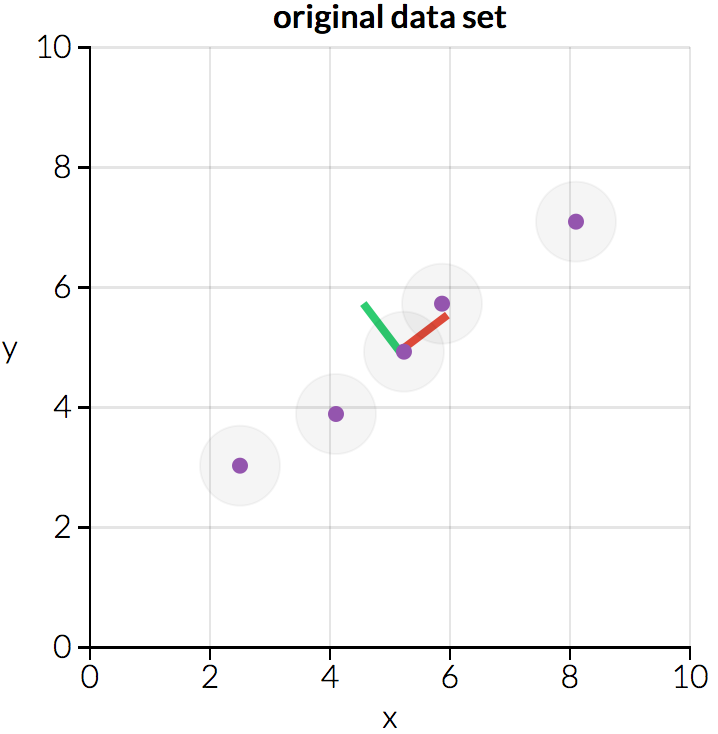
\includegraphics[width=0.45\textwidth]{pca_real_data}
    \caption{Example: Real Data with 2 Dimensions\cite{pca_visual}}
    \centering
    \label{subfig:pca_real_data}
\end{figure}

\begin{figure}[t!]
    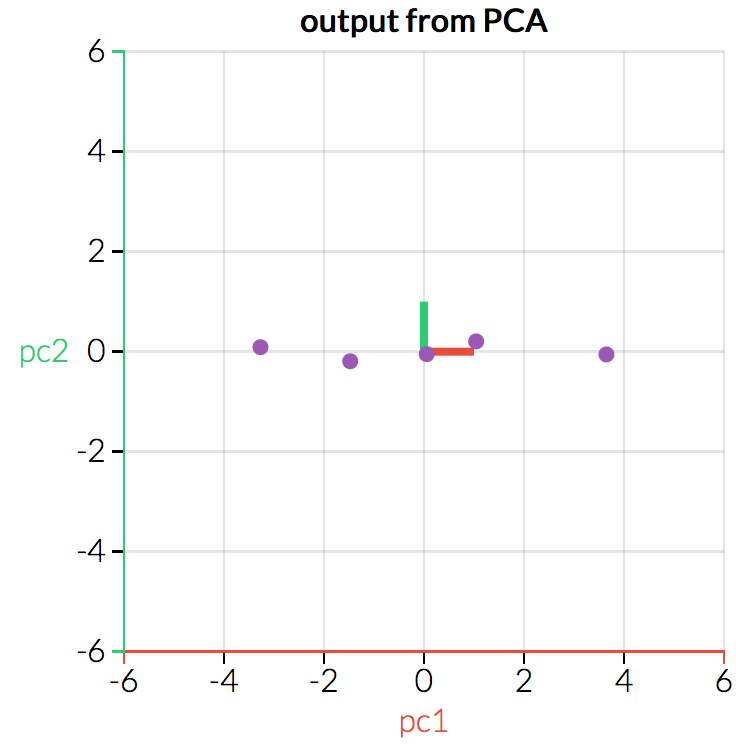
\includegraphics[width=0.45\textwidth]{pca_proj_data}
    \caption{Example: Data Projected on Eigen Plane\cite{pca_visual}}
    \centering
    \label{subfig:pca_proj_data}
\end{figure}
  
  We can also see from figure \ref{subfig:pca_proj_data} that maximum variance of data is along the \textbf{pc1 axis}. This makes the \textbf{pc1 axis} the 1st principal component of the data. Using this property of PCA we can choose the most important \textit{features} only from a data set while excluding the less important \textit{features}. We see from \textbf{figure} \ref{pca_real_data_on_axis}, real data needs both the \textbf{x and y plane} to represent the features (spread) of the data. On the other hand in \textbf{figure} \ref{pca_proj_data_on_axis} we can see that most of the variance for the data items has been condensed with negligible variance along the \textbf{pc2 axis}. All features of the data can now be abstracted onto the \textbf{pc1} plane. This method is the method we use for data abstraction while maintaining the features of the data set.% \ref{fig:pca_feature_set_abstraction} \ref{pca_proj_data_on_axis} \ref{pca_real_data_on_axis}
 
 \begin{figure}[t!]
    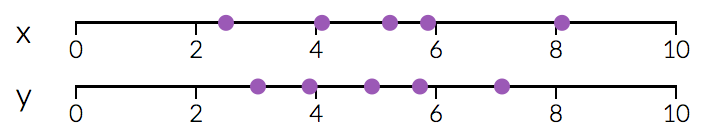
\includegraphics[width=0.45\textwidth]{pca_real_data_axis}
    \caption{Example: Variance for Real Data on X and Y axis individually}
    \centering
    \label{pca_real_data_on_axis}
\end{figure}

\begin{figure}[t!]
    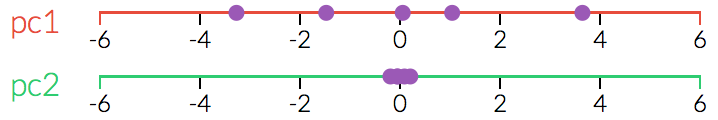
\includegraphics[width=0.45\textwidth]{pca_proj_data_axis}
    \caption{Example: Variance of Data on PCA axis individually}
    \centering
    \label{pca_real_data_on_axis}
\end{figure}
  
\subsubsection{Histogram Generation}
\label{hist_generation}
  Once the dimensionality of the data has been reduced using PCA, we need to reduce the point count ensuring we use the most dense distribution areas for data set comparisons. We tackle this problem by the use of Histograms.
Histogram is then generate on a per dimension \textit{(di)} basis with each dimension having 16 or 32 buckets with ranges computed as follows : 
\begin{equation}
     \begin{aligned}
       & bucket\_count = 16 \ or \ 32 \\
       & dim\_bucket\_range_{di}\ =\ max_{di} \ - \ min_{di}: \ \forall\ di\  in\ (1\ ..\ 3) \\
       & bucket\_size_{di} \ = \ dim\_bucket\_range_{di} \ / \    bucket\_count\ :\\
       & \forall\ di\ in\ (1\ ..\ 3) \\
       &  bucket\_range_j = [(bucket\_size * bucket_j + min_{di}),\\ 
       & \                  (bucketSize * (bucket_j + 1) + min_{di}))]; \\
       & \forall\ j\ in \ (1\ .. \ n)
     \end{aligned}
\end{equation}

This will give us the buckets with their ranges for all dimensions. We then proceed to generate \textit{three} histograms. Each data point is put into a bucket based on its value for that particular dimension. 
\textit{E.g.:} let \textit{three points} be represented in a 3-D Eigen plane by coordinates as follows: \\
$p1 = (1,\ 2,\ 3)$
$p2 = (-1,\ 0,\ 1)$
$p3 = (2,\ 3,\ 4)$ \\ 
Now, let there exist 2 buckets per dimension with Ranges as follows:  \\
$b_{11} = [-1,\ 2)$
$b_{12} = [2,\ 4)$
$b_{21} = [0, \ 2)$
$b_{22} = [2, \ 4)$
$b_{31} = [1, \ 3)$
$b_{32} = [3, \ 5)$ \\

Using the above points and bucket ranges we will now generate \textbf{3 Histograms}(one per dimension) with \textbf{2 buckets per histogram.} The histograms may be represented as follows: \\
\begin{itemize}
    \item Histogram for first dimension:\\
        $h\_points_1\ =\ {b_{11}\ :\  (p1,\  p2);\ b_{12}\ :\  (p3)\ };$
    
    \item Histogram for second dimension: \\
        $h\_points_2\ =\ {b_{21}\ :\  (p2);\ b_{22}\ :\  (p1, \ p3)\ };$
        
    \item Histogram for third dimension:\\
        $h\_points_3\ =  {b_{31}\ :\  (p2);\ b_{32}\ :\  (p1, \ p3)\ };$
\end{itemize}

Thus we can see from above example how each item becomes a part of a bucket if its coordinate for the given dimension lies in the bucket range for that dimension.

\subsubsection{Similarity Metric Computation}
\label{similarity_metric_calculation}
We now use the Welch's Test \cite{welch_test}\cite{boost_graph} to compute the probabilistic metric for similarity and to rank all history data sets wrt to each other and store in decreasing order of similarity. (Note: Will be used in run time historical reuse data set computation.) 
Welch test is computed for each dimension of the two sets being matched and the summation of the score for all three dimensions is as Similarity score for the two data set. Data sets are then ranked with each other based on the similarity score. Higher score means a better and match and vice versa.
\subsection{Training Algorithm}
This part of the algorithm is used to prepare and store data so as to have highest availability of reuse components for all candidates. We try and solve the challenges mentioned in \ref{chap-three} using the methods mentioned in \ref{overview}. 
Let our history database consist of "n" data sets named: $HD_1, HD_2, ... HD_n$.
The following Steps are done for each $HD_i \text{  for (i in 1 to n) } $:
\begin{itemize}
    \item \label{pca_gen_training} \textbf{PCA:} Compute Eigen vectors for $HD_i$ and project data on the Eigen vectors to normalize in Eigen plane and reduce dimensionality as shown in \ref{principal_comp_analysis}. We reduce all data into 3-D space for comparison purposes.
    \item \label{his_gen_training} \textbf{Histogram Generation:} Categorize PCA data for $HD_i$ buckets for histograms as shown in \ref{hist_generation}. One histogram is generated per dimension of data, thus we have a total of 3 histograms for each data set. Each histogram comprises of a total of 32 buckets. 
    \item \textbf{Relative Ranking:} Use Welch Test to rank all history data sets wrt to each other. Data sets are stored in decreasing order of similarity as shown in Algorithm \ref{hist_relative_ranking}. (Note: Will be used in run time historical reuse data set computation.)
    \item \textbf{Reuse Data for Data Set:} Run Algorithm of choice for Data Set and store \textit{Computation Reuse Data}. E.g.: In case of the K-means algorithm we choose the \textit{final centroids} computed by the K-Means Algorithm for current data set.
\end{itemize}

%==================================================================
%			History Rank ALGORITHM	BEGIN
% ==================================================================
\begin{algorithm}
\caption{History Data Sets- Relative Ranking}
\label{hist_relative_ranking}
\begin{algorithmic}[1]
\Procedure{RankHistoryData}{$History\_Database$}
\State $relative\_rank_{map}\ =\ ORDERED\_MAP(Similarity\_Score,\ Data\_Set)$
\State $score_{Final} = 0$
\For{each $HD_i$ in $History\_Database$}
	\For{each $HD_j$ in $History\_Database$ != $HD_i$}
		\State $score_{Final}$ = $ComputeSimilarity(HD_i,\ HD_j)$
		\State $relative\_rank_{map}.insert(score_{Final},\ HD_j)$
	\EndFor
	\State$(HD_i).Relative\_Ranking$ = $relative\_rank_{map}$
\EndFor
\EndProcedure
\end{algorithmic}
\end{algorithm}

%==================================================================
%			History Rank ALGORITHM	BEGIN
% ==================================================================

%==================================================================
%			Welch ALGORITHM	BEGIN
% ==================================================================
\begin{algorithm}
\caption{Similarity Metric Computation}
\label{similarity_computation}
\fontsize{10}{15}
\begin{algorithmic}[1]
\Procedure{ComputeSimilarity}{$D\_S_{Cur},\  D\_S_{Hist}\ $}
\State $score_{Final} = 0$
\State $Data_{CurDS} = TOP\_3\_BUCKET(D\_S_{Cur})$
\State $Data_{HistDS} = TOP\_3\_BUCKET(D\_S_{Hist})$
\For{each $dim_i$ in $Dimensions(D\_S_{Cur})$}
	\State $scr$ += $CalcWelchScr(Data_{CurDS}.colAt(dim_i),$\\
	\State $Data_{HistDS}.colAt(dim_i))$
\EndFor
\State\Return $scr$
\EndProcedure
\end{algorithmic}
\end{algorithm}


\subsubsection{Computing Best Match for Current Data-set (Run Time)}
This is the part of the algorithm that is actually responsible for the selection of the best match from the history data sets for the initialization for the current data set. This needs to be quick and accurate. Quick so that the overall overhead introduced by the selection process must not overshoot the total runtime improvements it may help us get, while the accuracy directly effects both the run time and the quality of clusters produced.

The two parts of the Matcher and Selector part of our algorithm may be defined as follows:
	\begin{itemize}
	\item \textbf{Screening:} This is the process where we select our initial candidates for the next step of our selection algorithm. This part of the algorithm essentially estimates the similarity in distribution for the current and corresponding historical data sets using the  Histograms generated in the previous steps. Variance Similarity is estimated as follows:			
		\begin{enumerate}
    			\item Take top-k most populated buckets for current data set and select corresponding top-k bins from all history data sets and top-k buckets with closest min and max to current data-set top-k bins.
		    \item Find ED for these data points between current data set and all historical data sets.
    			\item Choose Historical Data Sets with minimal distance as initial “Best Match” for both top-k buckets by rank and top-k buckets by range.
		\end{enumerate}
	Pseudo Code for an understanding of how our \textit{screening algorithm} runs can be seen in Algorithm \ref{screening_algo}.

%==================================================================
%			SCREENING ALGORITHM	BEGIN
% ==================================================================

 
\begin{algorithm}
\caption{Screening Algorithm}
\label{screening_algo}
\begin{algorithmic}[1]
\Procedure{Screening\textendash PrimaryCandidateSelection}{}
\State $least\_distance_{rank} = MAX$
\State $least\_distance_{range} = MAX$
\State $dim\_distance_{rank} = 0$
\State $dim\_distance_{range} = 0$
\State $HD\_Rank_{selected}$
\State $HD\_Range_{selected}$
\For {each $HD_x$ in History Database} 
	\For { each $Dim_i\  where\ i\  in\  1\  ..\  3\ $ }
		\For{each  $Bucket_j$ in Top 3 Buckets($Dim_i$) in Decreasing Order of Item Count for current data set} 
			\State 
			\For{each  $pt_{cd}$ and $pt_{HDi}$ in points($Bucket_j$)} 
				\State $distance_{rank}\ =\  dist(pt_{cd},\ pt_{HDi})$;
			\EndFor

			\State$Bucket_k$ = Bucket in $HD_i\  where\ range(bucket_k)\ \sim \  range(bucket_j)$
			
 	 		\For {each  $pt_{cd}\  in\ points(Bucket_j)\ $ \\ $and\ pt_{HDi}\ in\ Bucket_k$ } 
				\State $distance_{range}\ =\ dist(pt_{cd},\ pt_{HDi})$;  
			\EndFor
		\EndFor
 	 		
		\State $dim\_distance_{rank}\  =\  dim\_distance_{rank} \ + \ distance_{rank}$
		\State $dim\_distance_{range}\  =\  dim\_distance_{range} \ + \ distance_{range}$ 
	\EndFor
	\If{$dim\_distance_{rank}$ < $least\_distance_{rank}$}
 			\State $least\_distance_{rank}$ = $dim\_distance_{rank}$;
			\State $HD\_Rank_{selected}\ = \ HD_x$;
	\EndIf
   	 
	\If{$dim\_distance_{range}$ < $least\_distance_{range}$}
   		\State $least\_distance_{range}\ = dim\_distance_{range}$;
   	 	\State $HD\_Range_{selected}\ = \ HD_x$;
	\EndIf
\EndFor
\State\Return [$HD\_Rank_{selected}$, $HD\_Range_{selected}$]
\EndProcedure
\end{algorithmic}
\end{algorithm}


%==================================================================
%			SCREENING ALGORITHM	END
% %================================================================

%==================================================================
%			Best Match Computation ALGORITHM	BEGIN
% ==================================================================
 
\begin{algorithm}
\caption{Best Match Selection Algorithm}
\label{best_match_selection}
\fontsize{10}{15}
\begin{algorithmic}[1]
\Procedure{BestMatchSelection}{}
\State $primary\_candidates = Screening$\textendash$PrimaryCandidateSelection$
\State $BM\_score_{final} = INT_MIN$
\State $BM\_score_{cur}$ = $CompSim(DS_{cur},$ \\ $primary\_candidates[0])$
\State $BM_{data\_set} = primary\_candidates[0]$
\State $BM\_score_{cur}= CompSim(DS_{cur},$ \\ $primary\_candidates[1])$
\If{$BM\_score_{cur}\ >\ BM\_score_{final}$}
  \State $BM\_score_{final} = BM\_score_{cur}$
  \State $BM_{data\_set} = primary\_candidate[1]$
\EndIf
$PC\ =\ primary\_candidates;$
\For {each $HD_x$ in $TOP\_3_{rel\_rank}$($PC[0]$)} 
  \State $BM\_score_{cur} = CompSim(DS_{cur},\ HD_x)$
  \If{$BM\_score_{current}\ >\ BM\_score_{final}$}
    \State $BM\_score_{final} = BM\_score_{cur}$
    \State $best\_match_{data\_set} = HD_x$
  \EndIf
\EndFor

\For {each $HD_y$ in $TOP\_2\_{relative\_rank}$\\($PC[1]$)} 
  \State $BM\_score_{cur} =$ \\ $ CompSim(DS_{cur},\ HD_y)$
  \If{$BM\_score_{cur}\ >\ BM\_score_{final}$}
    \State $BM\_score_{final} = BM\_score_{cur}$
    \State $BM_{data\_set} = HD_y$
  \EndIf
\EndFor
\Return  $BM_{data_set}$
\EndProcedure
\end{algorithmic}
\end{algorithm}

%==================================================================
%			Best Match Computation ALGORITHM	END
% %================================================================
	\item \textbf{Find Best Match (Similarity Metric => Probabilistic Score):} 
	One we have found the best match candidates from out screening step, we simple calculate the Welch Test score for each dimension ($dim_i$) for each pair of current data set and chosen historic data sets.
		\begin{enumerate}
    			\item Find ``Similarity Metric`` as expalined in subsection \ref{sim_calc} and between current data set and above chosen “best match” data sets using Welch’s Test for all dimensions of all three data sets as shown in Algorithm \ref{similarity_computation}.
		    \item Similarly find “Similarity Metric” for top two relatively ranked data sets for current best match and top one for second best match.
		    \item Choose Data Set with highest Probability Score.
		\end{enumerate}
			Pseudo Code for an understanding of how our \textit{final selection algorithm} runs can be seen in Algorithm \ref{screening_algo}.	
	\item \textbf{Reuse Computations: }  In this section we use the computational data we had stored for history reuse in the training run for the historical data set selected. For instance, in the case of the K-Means algorithm, we now use the centroids from the chosen historical data set that were computed during the training run for historical data.
\end{itemize}

\subsubsection{Discussion}
Our final algorithm was reached at after a fair few trials and errors. Some of the major approaches used apart the latest approach for major challenges may be defined as below:
\subsubsection{Computation on Real Data and Incorrect Screening algorithm:}
\subsubsubsection{Implementation}
\begin{itemize}
    \item In this method I had initially use bin wise reduction on initial (real) data and then used PCA for dimension reduction of these reduced data points for the calculation of Eigen vectors and Eigen values only.
    \item I had then proceeded to run Student’s T-Test for relative ranking in training Run on real data.
    \item For Run Time computation I had used only the distance between the Eigen vectors for initial screening, choosing the data set with smallest difference in Eigen vectors as initial Best Match data set.
    \item I had then proceeded to Use Student T-Test on real data for computation of the probabilistic metric using all dimensions for the computation of the same.
    \item Python Numpy Libraries had been used for Student T-Test computation.
    \item History Reuse component Computations during training run was done on real data of historical data set instead of PCA data.
\end{itemize}

\subsubsubsection{Reasons for failure}
\begin{itemize}
    \item Data was not normalized thus computation would not be correct.
    \item Student T-Test worked only with Gaussian Distributions. Garbage value was returned for non Gaussian Data.
    \item Eigen Vectors of two data set may be orthogonal yet PDF (probability density function) may be close enough such as to generate similar clusters.
    \item Use of labels for direct initialization was flawed in the sense that if the data points were jumbled they would produce the wrong order of labels thus still providing a bad match.
    \item Bin Wise distribution of data points was an expensive operation and computation overhead increased with increase in dimensionality of data.
    \item Student T-Test had to compute for multiple dimensions of data and was a time expensive computation.
\end{itemize}

\subsubsection{Custom CPP Implementation for Welch’s Test}
Some of the earlier seen issues were corrected in this section as I noticed that a lot of the run time improvement was overshadowed by the time taken for choosing the historical data set. I also noticed that the Student T-Test was not reliable for non-Gaussian data and failed completely in case of different data set sizes.
This iteration was also mainly about ensuring quicker run time for the selection algorithm, so incremental updates were made to optimize the same. Some of the updates made may be enlisted as follows:
\begin{itemize}
    \item Implemented Custom Cpp implementation for Welch’s Test to over come overhead created by using python libraries for it and calling python script from Cpp.
    \item Removed the distribution of data into bins for data point reduction as it had a big overhead in computation and CPP Welch Test Libraries scaled well for larger data sets.
    \item Changed to use of Welch’s Test as compared to Student T-Test as Welch’s Test works with non Gaussian distributed data as well as compared to Student T-Test which makes assumptions of data distribution being Gaussian in nature.
    \item For Run Time computation I had used only the distance between the Eigen vectors for initial screening, choosing the data set with smallest difference in Eigen vectors as initial Best Match data set.
    \item Centroid Computation during training run was done on real data of historical data set instead of PCA data.
    \item Labels for Best Match historic data set were used as-is for current data set.
\end{itemize}

\subsubsection{Random Sampling for Order comparison.}
Experimentation on the approach showed non-reliable best match selection. Also I saw that often the best match might not even yield best results. One of the major reasons for this was the use of the incorrect use of historical data. For instance, in case of the K-Means algorithm the use of labels instead of the computed centroids lead to dependence on the order of the items in the historic data set. While the two data set may be similar and produce similar clusters, History Reuse with this method would still fail as initially the data points in current data set may get labeled incorrectly. I also realized that comparison of non-normalized data was in its very essence. I tried to correct the above issues with the following methodology:
\begin{itemize}
    \item Changed implementation to use of PCA data for most computations.
    \item Projected Historical data set points on Current Data Set Eigen Vectors. Used distance between data points of Current Data Set and historical data sets by randomly sampling 10\% of data sets against each other. Chose Data Set with minimum distance. This was done to try to use Historical data set with most point order similarity (and thus generated label order similarity) in conjunction with overall data set similarity.
    \item Welch’s Test was still used across all dimensions of actual data Similarity Metric Computation.
    \item Labels were used as-is for real data.
\end{itemize}
This implementation though corrected some of the above mentioned issues, it in its turn generated new issues:
\begin{itemize}
    \item Use of labels for direct initialization was flawed in the sense that if the data points were jumbled they would produce the wrong order of labels thus still providing a bad match.
    \item Random Sampling was a bad way to judge the order of the labels that would be generated by K-Means for data set.
    \item Eigen Vectors of two data set may be orthogonal yet PDF may be close enough such as to generate similar clusters.
\end{itemize}

\subsubsection{Use Of PCA Data for Welch’s Test and PCA data for centroid computation in Training Run:}
Experimentation still showed both the history reuse to be inconsistent and the overhead of computing historical data set was still quite large. I also realized that while Eigen Vectors of two data set may be orthogonal yet PDF might be close enough such as to generate similar clusters. To correct the above issues I used the following methods:
\begin{itemize}
    \item Used PCA data in training run for Centroid computation of historical data.
    \item Used PCA data for Welch’s Test based “Similarity Metric” computation.
    \item Still used labels from best match historical data set as initialization for current data set.
    \item Stopped projecting historical data sets data on current data set Eigen vectors, instead used self-projection, which could be done offline.
    \item Used Random Sampling for initial estimation of best match data set.
\end{itemize}
The use of Labels was still flawed. Also the use of random sampling was not a very effective methodology for screening as it would often lead to the selection of bad candidates.

\section{Evaluations}
\label{chap-five}

\subsection{Methodology}
We have used leave-one cross testing for all experimentations. Most data sets for experimentation are stock databases available on the UCI machine-learning repository while some source data sets are Microsoft released source data sets for machine learning.
These data sources are then divided into data sets. Depending on the size of the data source\cite{uci_machine_repo} we may have any where between 10 to 43 data sets, where in all save one are treated as historic data sets. We have also allowed all algorithms to converge to the same epsilon error rate thus ensuring the run time comparison for similar quality output for algorithms.
All experiments have been carried out on Octa core Intel Xeon CPU E5-2650 Running Ubuntu Linux 14.04 LTS with 16GB of RAM.
\subsection{Experiments}
To demonstrate the efficacy and efficiency of our program we evaluate our approach by testing it on various large real world data-sets and compare our algorithm to two most frequently used and vastly accepted K-Means initialization algorithms: standard K-Means (Random Select initialization also known as Lloyd's Algorithm) and K-Means++ initialization (Weighed Probability based initialization based on squared of distance from initial randomly selected center). Both the above algorithms are implemented in the OpenCV library, which has been used as the standard library for Lloyd’s Algorithm implementation. We run all three algorithms on the same data sets with the same error rate for convergence.
We have also compared the historical data-set selected by our algorithm to all other data-sets available in history to show the accuracy of our algorithm in selecting the best available data-set.

\begin{figure}[t!]
    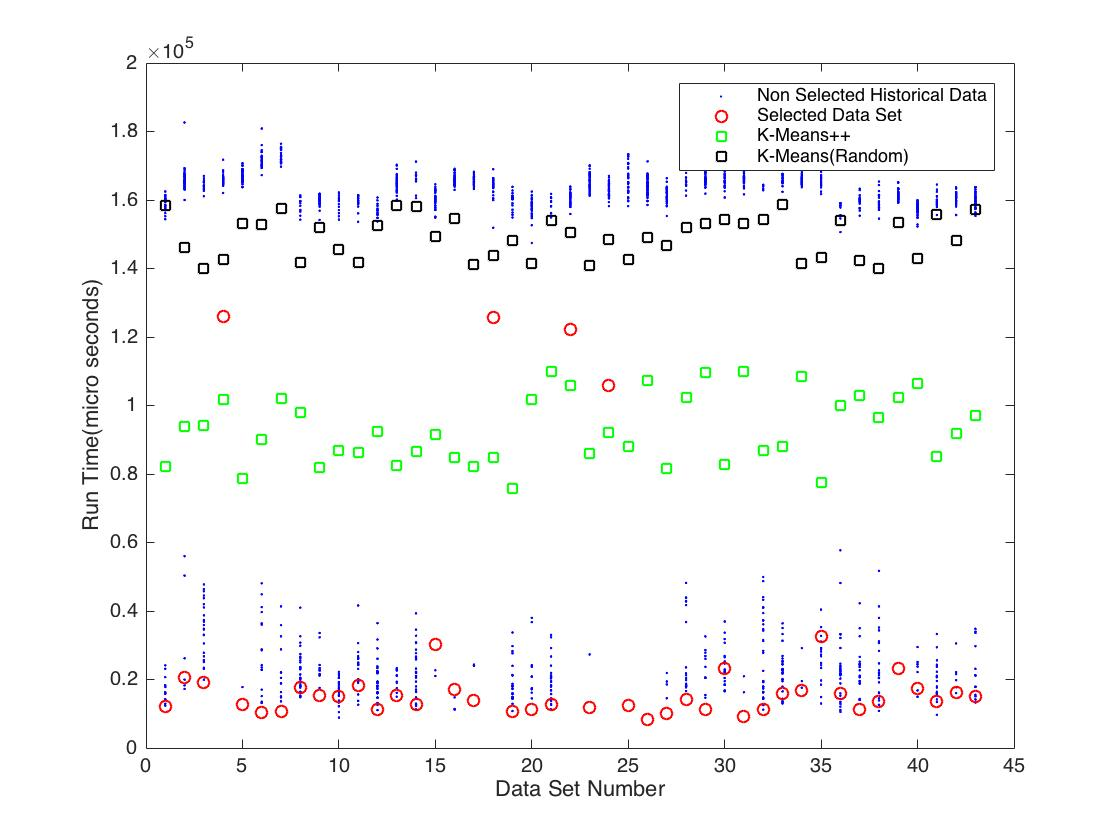
\includegraphics[width=\textwidth, height=7cm,keepaspectratio]{road_240}
    \caption{Hit-Rate (Road Network k=120)}
    \centering
    \label{fig:gas_240_selection}
\end{figure}

\begin{figure}[t!]
    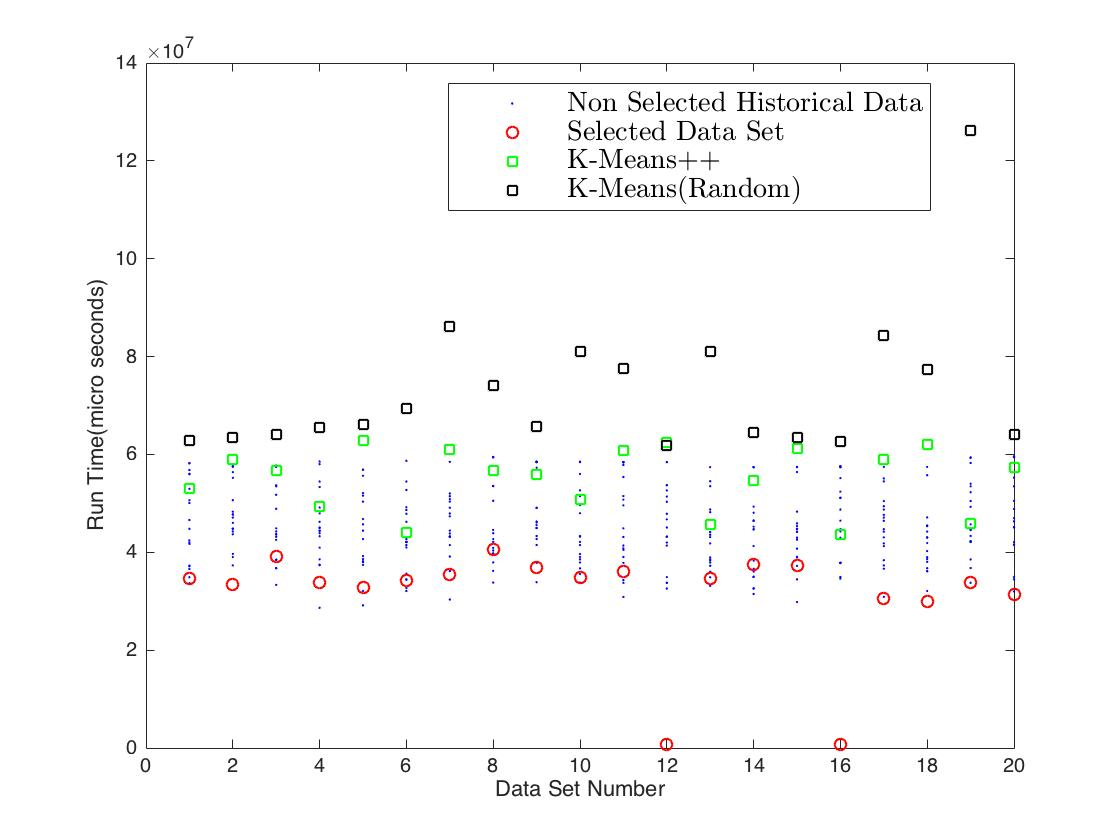
\includegraphics[width=\textwidth, height=7cm,keepaspectratio]{nnData_600}
    \caption{Hit-Rate (Caltec 101 for k=600)}
    \centering
    \label{fig:caltec_600_selection}
\end{figure}

\setlength{\arrayrulewidth}{0.2mm}
\setlength{\tabcolsep}{10pt}
%\renewcommand{\arraystretch}{1}
\begin{table*}[h!]
% \begin{minipage}{\textwidth}
\centering
% \begin{center}
\begin{tabular}{|l|c|c|c|r|}
\hline\hline
    \textbf{Data-set Name} & \textbf{History Data-set cnt.} & \textbf{Cluster Count} & \textbf{Top 5 cnt} & \textbf{Hit Rate \%} \\
\hline\hline
    \textbf{Road Network}   & 43 &
    \begin{tabular}{c} 40 \\ 80 \\ 120 \\ 240 \end{tabular} &
    \begin{tabular}{c} 42 \\ 41 \\ 43 \\ 43 \end{tabular} &
    \begin{tabular}{c} 97.67\% \\ 95.34\% \\ 100\% \\ 100\% \end{tabular} \\
\hline
    \textbf{Kegg Network}   & 10 &
    \begin{tabular}{c} 40 \\ 80 \\ 120 \\ 240 \end{tabular} &
    \begin{tabular}{c} 8 \\ 9 \\ 8 \\ 8 \end{tabular} &
    \begin{tabular}{c} 80\% \\ 90\% \\ 80\% \\ 80\% \end{tabular} \\
\hline
    \textbf{US Gas Sensor Data}   & 36 &
    \begin{tabular}{c} 40 \\ 80 \\ 120 \\ 240 \end{tabular} &
    \begin{tabular}{c} 28 \\ 29 \\ 29 \\ 28 \end{tabular} &
    \begin{tabular}{c} 77.7\% \\ 80.5\% \\ 80.5\% \\ 77.7\% \end{tabular} \\
\hline
    \textbf{NotreDame}   & 20 &
    \begin{tabular}{c} 40 \\ 80 \\ 120 \\ 240 \end{tabular} &
    \begin{tabular}{c} 17 \\ 18 \\ 17 \\ 17 \end{tabular} &
    \begin{tabular}{c} 85\% \\ 90\% \\ 85\% \\ 85\% \end{tabular} \\
\hline
    \textbf{Tiny}   & 20 &
    \begin{tabular}{c} 80 \\ 120 \\ 240 \\ 360 \\ 480 \\ 600 \end{tabular} &
    \begin{tabular}{c} 20 \\ 18 \\ 16 \\ 17 \\ 18 \\ 18 \end{tabular} &
    \begin{tabular}{c} 100\% \\ 90\% \\ 80\% \\ 85\% \\ 90\% \\ 90\% \end{tabular} \\
\hline
    \textbf{Uk Bench}   & 20 &
    \begin{tabular}{c} 80 \\ 120 \\ 240 \\ 360 \\ 480 \\ 600 \end{tabular} &
    \begin{tabular}{c} 20 \\ 18 \\ 16 \\ 17 \\ 18 \\ 18 \end{tabular} &
    \begin{tabular}{c} 100\% \\ 90\% \\ 80\% \\ 85\% \\ 90\% \\ 90\% \end{tabular} \\
\hline
    \textbf{Caltec 101}   & 20 &
    \begin{tabular}{c} 80 \\ 120 \\ 240 \\ 360 \\ 480 \\ 600 \end{tabular} &
    \begin{tabular}{c} 20 \\ 18 \\ 16 \\ 17 \\ 18 \\ 18 \end{tabular} &
    \begin{tabular}{c} 100\% \\ 90\% \\ 80\% \\ 85\% \\ 90\% \\ 90\% \end{tabular} \\
\hline
\end{tabular}
\caption{Selection Hit Rate K-Means History Reuse}
\label{table:1}
% \end{center}
\end{table*}

\textbf{Consistent Selection of Best Match Historical Data-set from History:} The experiments run, show that our algorithm is able to consistently able to select one of the top 5 data-sets for history reuse from available historical data-sets. By consistent, we mean that our algorithm is able to select one of the top 5 available data sets with hit rate of above seventy percent across data sets irrespective of the size and the cluster count. This is expected as we aim to compare data set based on similarity while the cluster count is not taken into consideration in the matching process. \textbf{\textit{Table \ref{table:1}}} shows the hit rate for our algorithm.
We can clearly see from the table that our algorithm is able to select one of the top 5 best data sets for historical reuse from the available data sets consistently irrespective of the cluster count and the total historically available data sets. 
This thus validates our theory for probabilistic selection for matching data sets using the \textbf{Welch's Test} for null hypothesis testing for similarity of data sets. We are also able to see clearly that our selection criteria continues to perform well across a wide range of cluster counts and thus validates our hypothesis that data-set similarity should be used as the primary measure to gauge quality of data-set for history reuse without the explicit need for taking into account the total number of clusters \textit{(k)} the data-set is to be clustered into. We have chosen to limit the total number of clusters to 256 so as to have meaningful clusters for data sets of relatively small sizes.
Columns 3, 4 and 5 show us how well our data-set selection algorithm works across various cluster indexes and also how little variation is seen in the performance of the data-sets selected by our algorithm irrespective of the number of clusters \textit{(k)}. We also show that our hit rate is a minimum of 70 percent (Some error is to be expected as the selection algorithm works on probabilistic model for making best guess.)
Figures \ref{fig:gas_240_selection} and \ref{fig:caltec_600_selection} show how our selected historical data set performs in comparison to all other data sets available for selection in our history database. We  see from them, the accuracy of algorithm in consistently choosing one of the best match data sets from history with high accuracy (>~ 75\%). We see that our algorithm chooses either the best match data set or data set close to best match. This proves the accuracy of our algorithm.
\textbf{Consistent Scalable approach to Selection:} Our experiments also show that our method scales well with the increase in dimensionality of data \textit{(d)}, the size of the data-set\textit{(n)} and the cluster count\textit{(k)}. \textbf{\textit{Figures \ref{fig:selection_overhead} and \ref{fig:selection_overhead_large}}} show our experimental results for various data sets with varying dimensionality and sizes. These figures clearly show that for any given data set the selection time is completely independent of the cluster count \textit{(k)}. This is in complete contrast to both the  \textit{random K-Means (Lloyd's Algorithm)} and the K-Means++ algorithm where the initialization overhead is directly proportional to the cluster count \textit{(k)} for the data set. Our experimental results also serve the purpose of showing us that our initialization methodology has an over head very small compared to the total run time of the algorithm even for the smallest of chosen cluster counts. This combined with the proven choosing of better initialization centroids (as seen in Table \ref{table:total_runtime_comparison} and Table \ref{table:iteration_comparison} which show an overall improvement in both run time as well as the number of iterations taken for the data to converge) gives us a win-win situation of a comprehensively better initialization methodology in comparison to both the previously mentioned methods.


\begin{figure}[t!]
    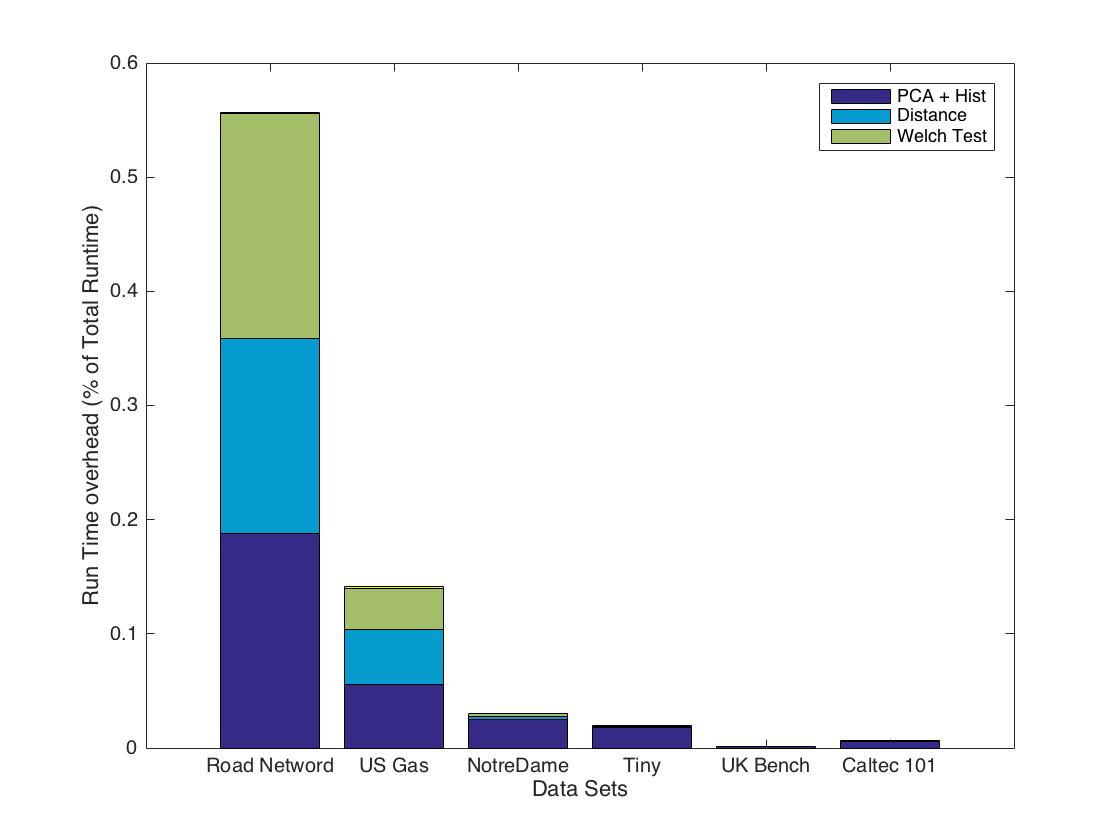
\includegraphics[width=\textwidth , height=7cm,keepaspectratio]{stacked_overhead}
    \caption{Best Match Selection Overhead (Maximum for Small \textit{k})}
    \centering
    \label{fig:selection_overhead}
\end{figure}

\begin{figure}[t!]
    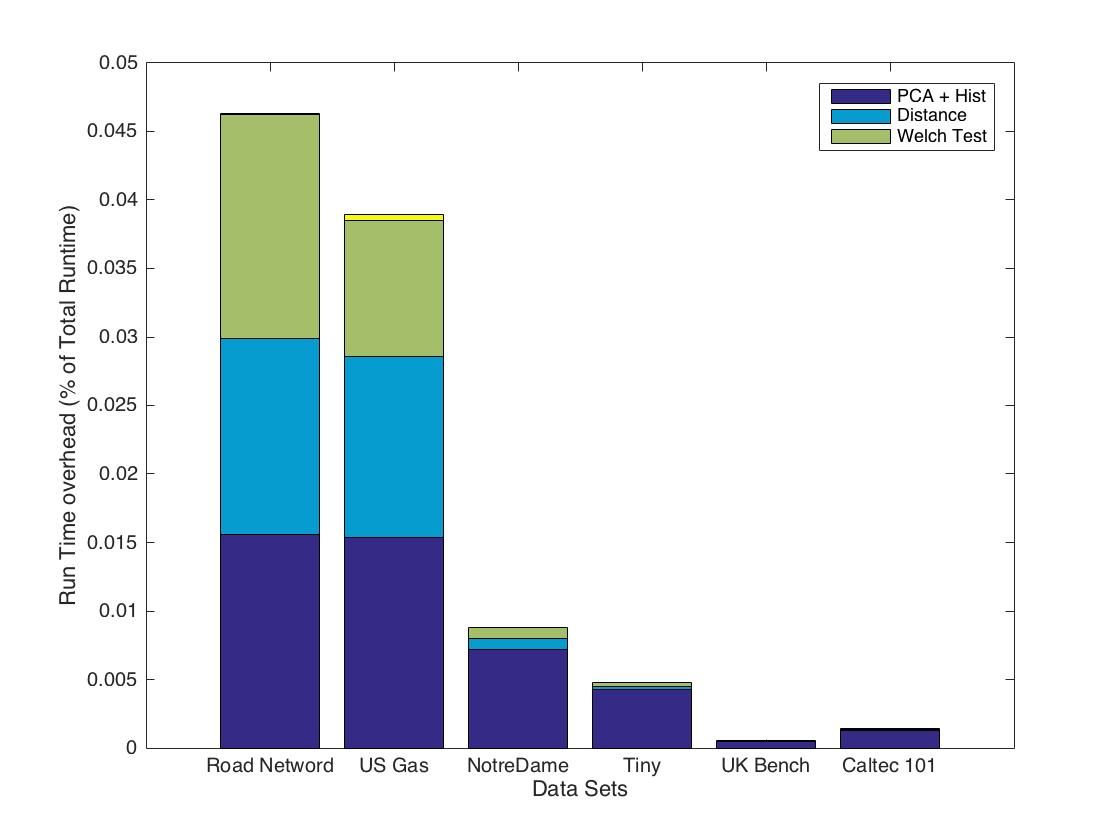
\includegraphics[width=\textwidth , height=7cm,keepaspectratio]{stacked_overhead_large}
    \caption{Best Match Selection Overhead (Minimum for Large \textit{k})}
    \centering
    \label{fig:selection_overhead_large}
\end{figure}

\begin{figure}[b!]
    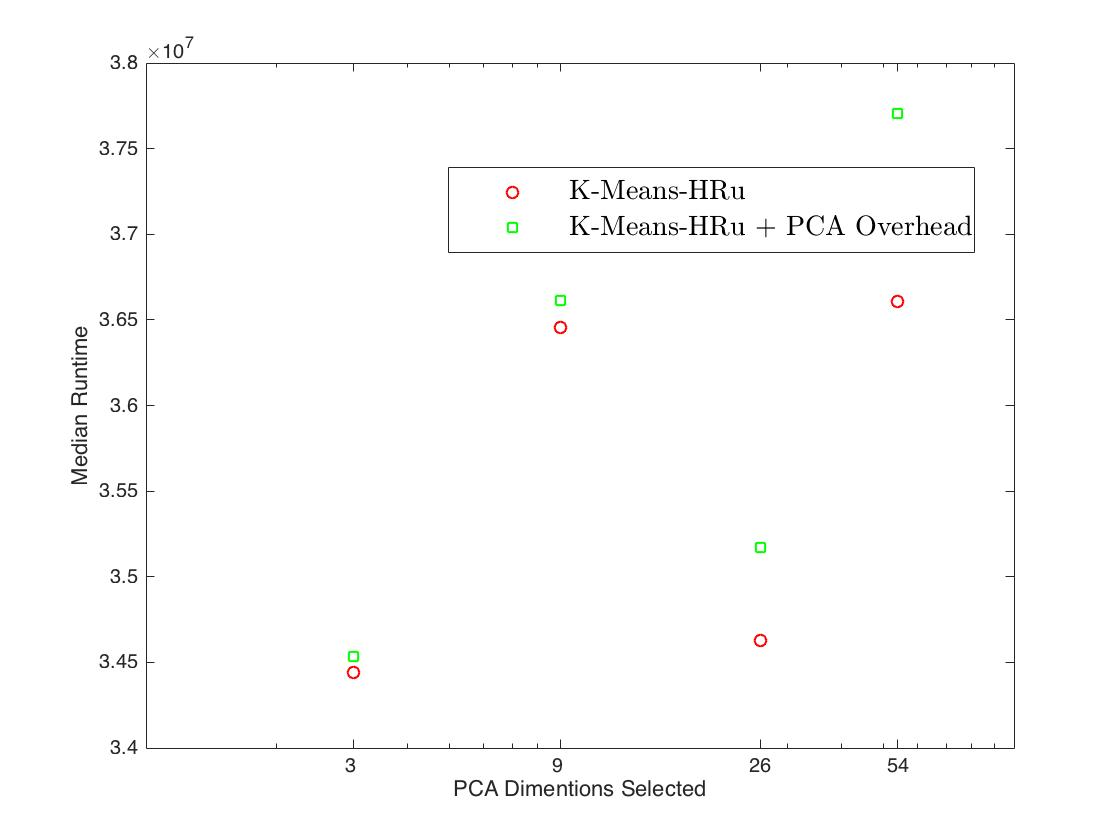
\includegraphics[width=\textwidth , height=7cm,keepaspectratio]{PCA_results}
    \caption{Performance for various PCA Dimension Count(Caltec 101; K = 600). Default PCA Dims: 3}
    \centering
    \label{fig:pca_overhead}
\end{figure}

Referencing the above mentioned tables and figures, we can also see that our selection mechanism takes only a very small percentage of the total run time for the algorithm for larger data sets (<~0.1\%) and while it may be a significant part of the initialization for smaller data sets the quality improvement in the initialization centroids is sufficient to offset the run time for the algorithm to be a viable initialization methodology for all data sets of varying sizes. 
Though speed up using our methodology is seen in all cases, it is best suited for larger data sets, as in that case our overhead for history best match selection almost becomes negligible.

From \textit{\textbf{Figure \ref{fig:pca_overhead}}} we can also see that even while retaining higher variances for historic data sets, no further speedup is seen in run time while the introduced overhead becomes a significant percentage for the total run time and may lead to further overheads as data set sizes increase.

\bgroup
\setlength{\arrayrulewidth}{0.2mm}
\setlength{\tabcolsep}{10pt}
\renewcommand{\arraystretch}{1}
\begin{table*}[t!]
\begin{minipage}{\textwidth}
\centering
%\begin{top}
\begin{tabular}{|l|c|c|c|c|c|c|r|}
\hline\hline
    \textbf{Data-set} & \textbf{n} & \textbf{d} & \textbf{k} & \textbf{K-Means (Time $\mu$S)} & \textbf{K-Means++} & \textbf{K-Means-HRU}\\
\hline\hline
    \textbf{Road Net.}   & 1.0E4 & 3 &
    \begin{tabular}{c} 40 \\ 80 \\ 120 \\ 240 \end{tabular} &
    \begin{tabular}{c} 8.5E4 \\ 1.6E5 \\ 2.01E5\\ 2.4E5\\ \end{tabular}&
    \begin{tabular}{c} 1.7X \\ 2.4X \\ 2.2X \\ 1.8X \\ \end{tabular} &
    \begin{tabular}{c} 6.7X \\ 10.0X \\ 10.0X \\1.6X \\ \end{tabular}\\
\hline
    \textbf{Kegg Net.}   & 2.0E4 & 10 &
    \begin{tabular}{c} 40 \\ 80 \\ 120 \\ 240 \end{tabular} &
    \begin{tabular}{c} 1.9E5 \\ 2.8E6 \\ 3.9E5 \\ 6.3E5 \\ \end{tabular} &
    \begin{tabular}{c}  2.5X \\ 1.9X \\ 1.6X \\ 1.9X \\ \end{tabular}&
    \begin{tabular}{c} 2X \\ 2.2X \\  2.8X \\ 3.2X \\ \end{tabular}\\
\hline
    \textbf{US Gas}   & 1.45E4 & 13 &
    \begin{tabular}{c} 40 \\ 80 \\ 120 \\ 240 \end{tabular} &
    \begin{tabular}{c} 3.2E5 \\ 4.7E5 \\ 5.2E5 \\ 8.9E5 \end{tabular} &
    \begin{tabular}{c} 2.4X \\ 1.9X \\ 1.9X \\ 1.7X \\  \end{tabular}&
    \begin{tabular}{c} 5.6X \\ 4.4X \\ 3.9X \\ 4.3X \\ \end{tabular}\\
\hline
    \textbf{NotreDame}   & 1.45E4 & 13 &
    \begin{tabular}{c} 40 \\ 80 \\ 120 \\ 240 \\ \end{tabular} &
    \begin{tabular}{c} 2.1E6 \\ 3.8E6 \\ 5.5E6 \\ 1.02E6\\ \end{tabular} &
    \begin{tabular}{c} 1.2X \\ 1.3X \\ 1.3X \\ 1.4X \\ \end{tabular}&
    \begin{tabular}{c} 2.4X \\ 2.3X \\ 2.3X \\ 2.3X \\ \end{tabular}\\
\hline
    \textbf{Tiny}   & 1.45E4 & 13 &
    \begin{tabular}{c} 80 \\ 120 \\ 240 \\ 360 \\ 480 \\ 600 \end{tabular} &
    \begin{tabular}{c} 0.9E8 \\ 1.3E8 \\ 2.5E8 \\ 3.2E8 \\ 3.9E8 \\ 4.3E8 \\ \end{tabular} &
    \begin{tabular}{c} 1.4X \\ 1.6X \\ 2.1X \\ 2.0X \\ 2.9X \\ 2.9X \\ \end{tabular}&
    \begin{tabular}{c} 2.8X \\ 2.9X \\ 3.8X \\ 2.7X \\ 4.1X \\ 4.1X \\  \end{tabular}\\
\hline
    \textbf{Uk Bench}   & 1.45E4 & 13 &
    \begin{tabular}{c} 80 \\ 120 \\ 240 \\ 360 \\ 480 \\ 600 \end{tabular} &
    \begin{tabular}{c} 1.7E7 \\ 2.3E7 \\ 4.2E7 \\ 4.7E7 \\ 5.8E7 \\ 6.8E7 \\ \end{tabular} &
    \begin{tabular}{c} 1.1X \\ 1.2X \\ 1.4X \\ 1.25X \\ 1.4X \\ 1.3X \\ \end{tabular}&
    \begin{tabular}{c} 2.7X \\ 2.5X \\ 2.5X \\ 2.4X \\ 2.1X \\ 2.3X \\ \end{tabular}\\
    
\hline
    \textbf{Caltec 101}   & 1.45E4 & 13 &
    \begin{tabular}{c} 80 \\ 120 \\ 240 \\ 360 \\ 480 \\ 600 \end{tabular} &
    \begin{tabular}{c} 1.9E7 \\ 2.2E7 \\ 4.2E7 \\ 5.3E7 \\ 6.5E7 \\ 7.3E7 \\ \end{tabular} &
    \begin{tabular}{c} 1.2X \\ 1.1X \\  1.4X \\ 1.4X \\   1.3X \\ 1.3X \\ \end{tabular}&
    \begin{tabular}{c} 2.6X \\ 2.1X \\ 2.3X \\ 2.3X \\ 2.2X \\ 2.1X \\ \end{tabular}\\
\hline
\end{tabular}
\caption{Runtime comparison: K-Means, K-Means++ and K-Means-HRU \textit{(*All times in $\mu$S)}}
\label{table:total_runtime_comparison}
%\end{top}
\end{minipage}
\end{table*}
\egroup

\textbf{Consistent Speed up for K-Means algorithm:} The end requirement of any initialization algorithm is to ensure that we achieve a consistent speed up over previous approaches. While running our initialization algorithm for K-Means we were able to see consistent speed up in run-time of algorithm as compared to both K-Means and K-Means++ algorithm for all data sets across a wide range of cluster counts ranging from 40 to 600. This is though dependent on quality of historical data sets available. A bad match may lead to relatively bad starting points which in turn leads to an increase in time taken for convergence. Not withstanding the above argument we were able to see consistently good performance by our algorithm for real data sets. This is largely due to the normalization of the data sets using the PCA based approach and then using cluster information based on this normalized data rather than the actual data. This also removes the need for the data to have Gaussian distribution. This gives a higher chance of finding a better historical match, thus giving consistent speed up over various data sets with different dimensionality\textit{(d)} and different cardinality\textit{(n)} for varying cluster counts \textit{k}.

Figures \ref{fig:box_speedup_small} and \ref{fig:box_speedup_large} shows the range of speed up across various data sets with varying degrees of freedom as well as different dimensionality for the same cluster counts. We can clearly see from the graphs that our algorithm consistently outperforms both the \textit{random K-Means(Lloyd’s Algorithm)} and the \textit{K-Means++ algorithm} in run time performance.


\begin{figure*}[p!]
    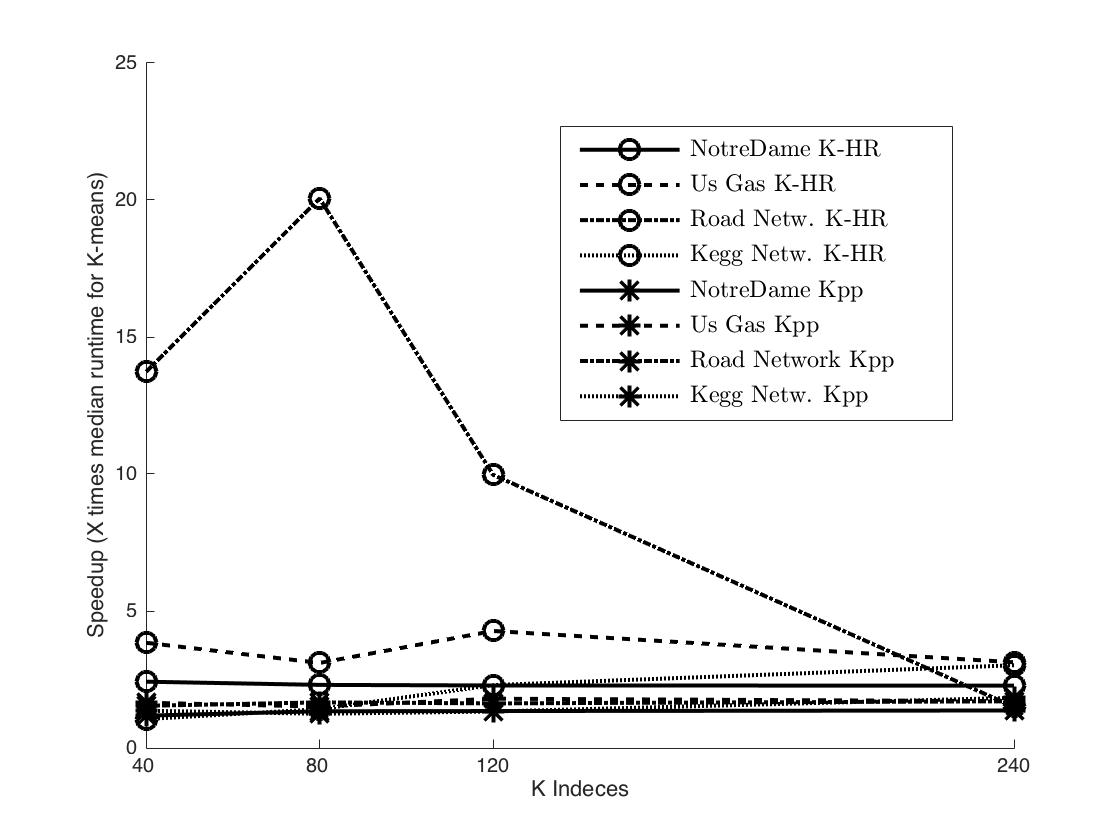
\includegraphics[width=\textwidth]{k_means_speedup_line_small}
    \caption{Median Speed up, Small Data (k=240)}
    \centering
    \label{fig:line_speedup_small}
\end{figure*}

\begin{figure*}[h!]
    \centering
        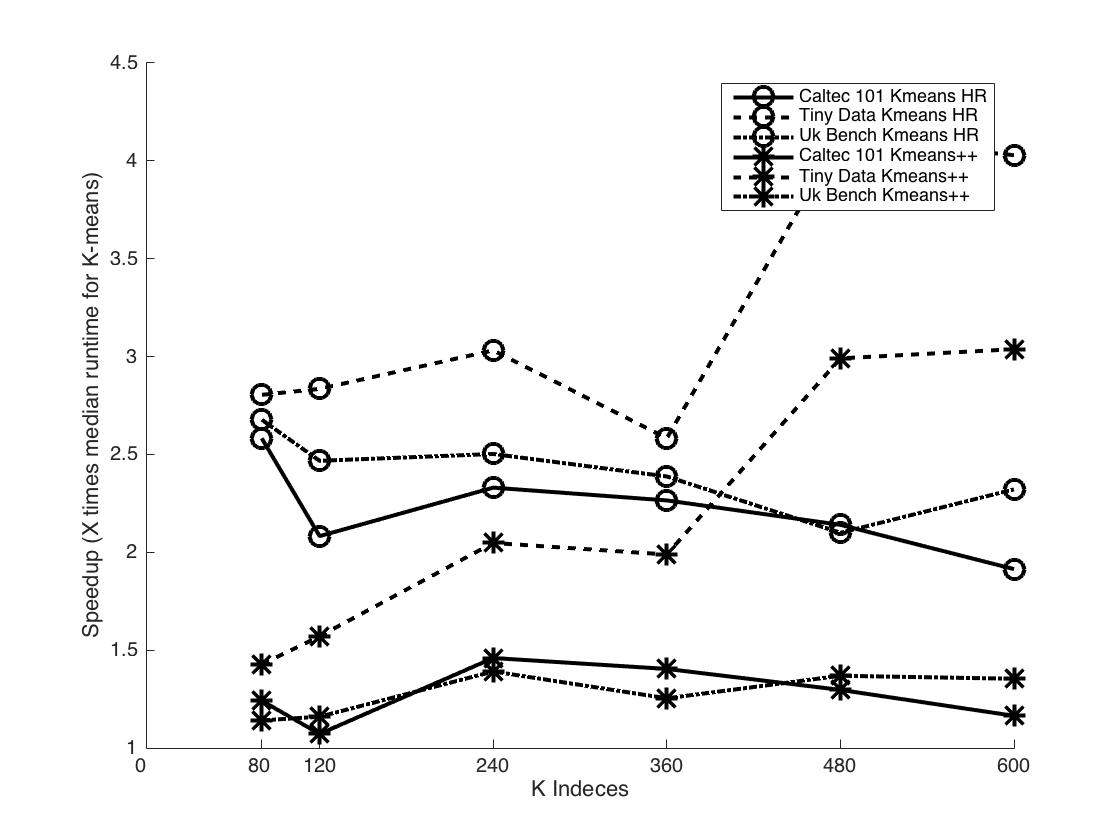
\includegraphics[width=\textwidth, height=10cm,keepaspectratio]{k_means_speedup_line_large}
    \caption{Median Speed up, Large Data (k=600)}
    \label{fig:line_speedup_large}
\end{figure*}

Figures \ref{fig:line_speedup_small} and \ref{fig:line_speedup_large} depict the speed up seen by our algorithm over various cluster sizes for all data sets. We can see that the general trend is that speed up seen is in general higher for larger cluster count. This is particularly true because as the cluster count increases we see a speed up in both the initialization method as well as the actual run time because of the improvement seen in the initialization centroids.

\setlength{\arrayrulewidth}{0.2mm}
\setlength{\tabcolsep}{10pt}
\renewcommand{\arraystretch}{1}
\begin{table*}[t!]
\begin{minipage}{\textwidth}
\centering
%\begin{top}
\begin{tabular}{|l|c|c|c|c|c|c|r|}
\hline\hline
    \textbf{Data-set} & \textbf{n} & \textbf{d} & \textbf{k} & \textbf{K-Means (Random)} & \textbf{K-Means++} & \textbf{K-Means-HRu}\\
\hline\hline
    \textbf{Road Net.}   & 1.0E4 & 3 &
    \begin{tabular}{c} 40 \\ 80 \\ 120 \\ 240 \end{tabular} &
    \begin{tabular}{c} 128 \\ 119 \\ 110 \\ 102 \\ \end{tabular}&
    \begin{tabular}{c} 69 \\ 52 \\ 46 \\ 79 \\ \end{tabular} &
    \begin{tabular}{c} 39 \\ 27 \\ 30 \\ 82 \\ \end{tabular}\\
\hline
    \textbf{US Gas}   & 1.45E4 & 13 &
    \begin{tabular}{c} 40 \\ 80 \\ 120 \\ 240 \end{tabular} &
    \begin{tabular}{c} 117 \\ 111 \\ 106 \\ 100 \\ \end{tabular} &
    \begin{tabular}{c} 58 \\ 59 \\ 58 \\ 55 \\ \end{tabular}&
    \begin{tabular}{c} 26 \\ 32 \\ 33 \\ 37\\ \end{tabular}\\
\hline
    \textbf{NotreDame}   & 1.45E4 & 13 &
    \begin{tabular}{c} 40 \\ 80 \\ 120 \\ 240 \\ \end{tabular} &
    \begin{tabular}{c} 162 \\ 154 \\ 132 \\ 103 \\ \end{tabular} &
    \begin{tabular}{c} 142 \\ 114.5 \\ 101 \\ 74 \\ \end{tabular}&
    \begin{tabular}{c} 69.5 \\ 65 \\ 60 \\ 48.5 \\ \end{tabular}\\
\hline
    \textbf{Tiny}   & 1.45E4 & 13 &
    \begin{tabular}{c} 80 \\ 120 \\ 240 \\ 360 \\ 480 \\ 600 \end{tabular} &
    \begin{tabular}{c} 195 \\ 181.5 \\ 168.5 \\ 129.5 \\ 119.5 \\ 111.5 \\ \end{tabular} &
    \begin{tabular}{c} 164 \\ 154.5 \\ 120.5 \\ 99.5 \\ 87.5 \\ 72 \\ \end{tabular}&
    \begin{tabular}{c} 108 \\ 98 \\ 87.5 \\ 74 \\ 67 \\ 58 \\ \end{tabular}\\
\hline
    \textbf{Uk Bench}   & 1.45E4 & 13 &
    \begin{tabular}{c} 80 \\ 120 \\ 240 \\ 360 \\ 480 \\ 600 \end{tabular} &
    \begin{tabular}{c} 274.5 \\ 273.5 \\ 251 \\ 233 \\ 216 \\ 196 \\ \end{tabular} &
    \begin{tabular}{c} 191 \\ 174.5 \\ 121 \\ 102 \\ 79.5 \\ 72 \\ \end{tabular}&
    \begin{tabular}{c} 85.5 \\ 82 \\ 75 \\ 70.5 \\ 63.5 \\ 57.5 \\ \end{tabular}\\
    
\hline
    \textbf{Caltec 101}   & 1.45E4 & 13 &
    \begin{tabular}{c} 80 \\ 120 \\ 240 \\ 360 \\ 480 \\ 600 \end{tabular} &
    \begin{tabular}{c} 219.5 \\ 171 \\ 178 \\ 146.5 \\ 137 \\ 108 \\ \end{tabular} &
    \begin{tabular}{c} 175.5 \\ 156.5 \\ 116.5 \\ 100 \\ 90 \\ 79 \\ \end{tabular}&
    \begin{tabular}{c} 84.5 \\ 80.5 \\ 74 \\ 69 \\ 61 \\ 58.5 \\ \end{tabular}\\
\hline
\end{tabular}
\caption{Median Iteration count comparison for K-Means, K-Means++ and K-Means with History Reuse.}
\label{table:iteration_comparison}
%\end{top}
\end{minipage}
\end{table*}

Results seen in Figures \ref{fig:selection_overhead} and \ref{fig:selection_overhead_large}  and Table \ref{table:total_runtime_comparison} together also show us that the speed ups are consistent irrespective of the cluster counts \textit{(k)} in terms of both the run time of the algorithms and the number of iterations taken for the convergence of the algorithm to similar error rate. This is again an intuitive results which confirms our hypothesis: a consistent selection methodology independent of the cluster index size would lead to sizable improvement in run time. This is so because run time improvement is seen in both the initialization overhead as well as the actual run time of the algorithm. As the cluster count\textit{(k)} increases, the amount of initialization overhead for both the above mentioned initialization methodology becomes a significant part of the total run time for the algorithm.

\begin{figure}[t!]
    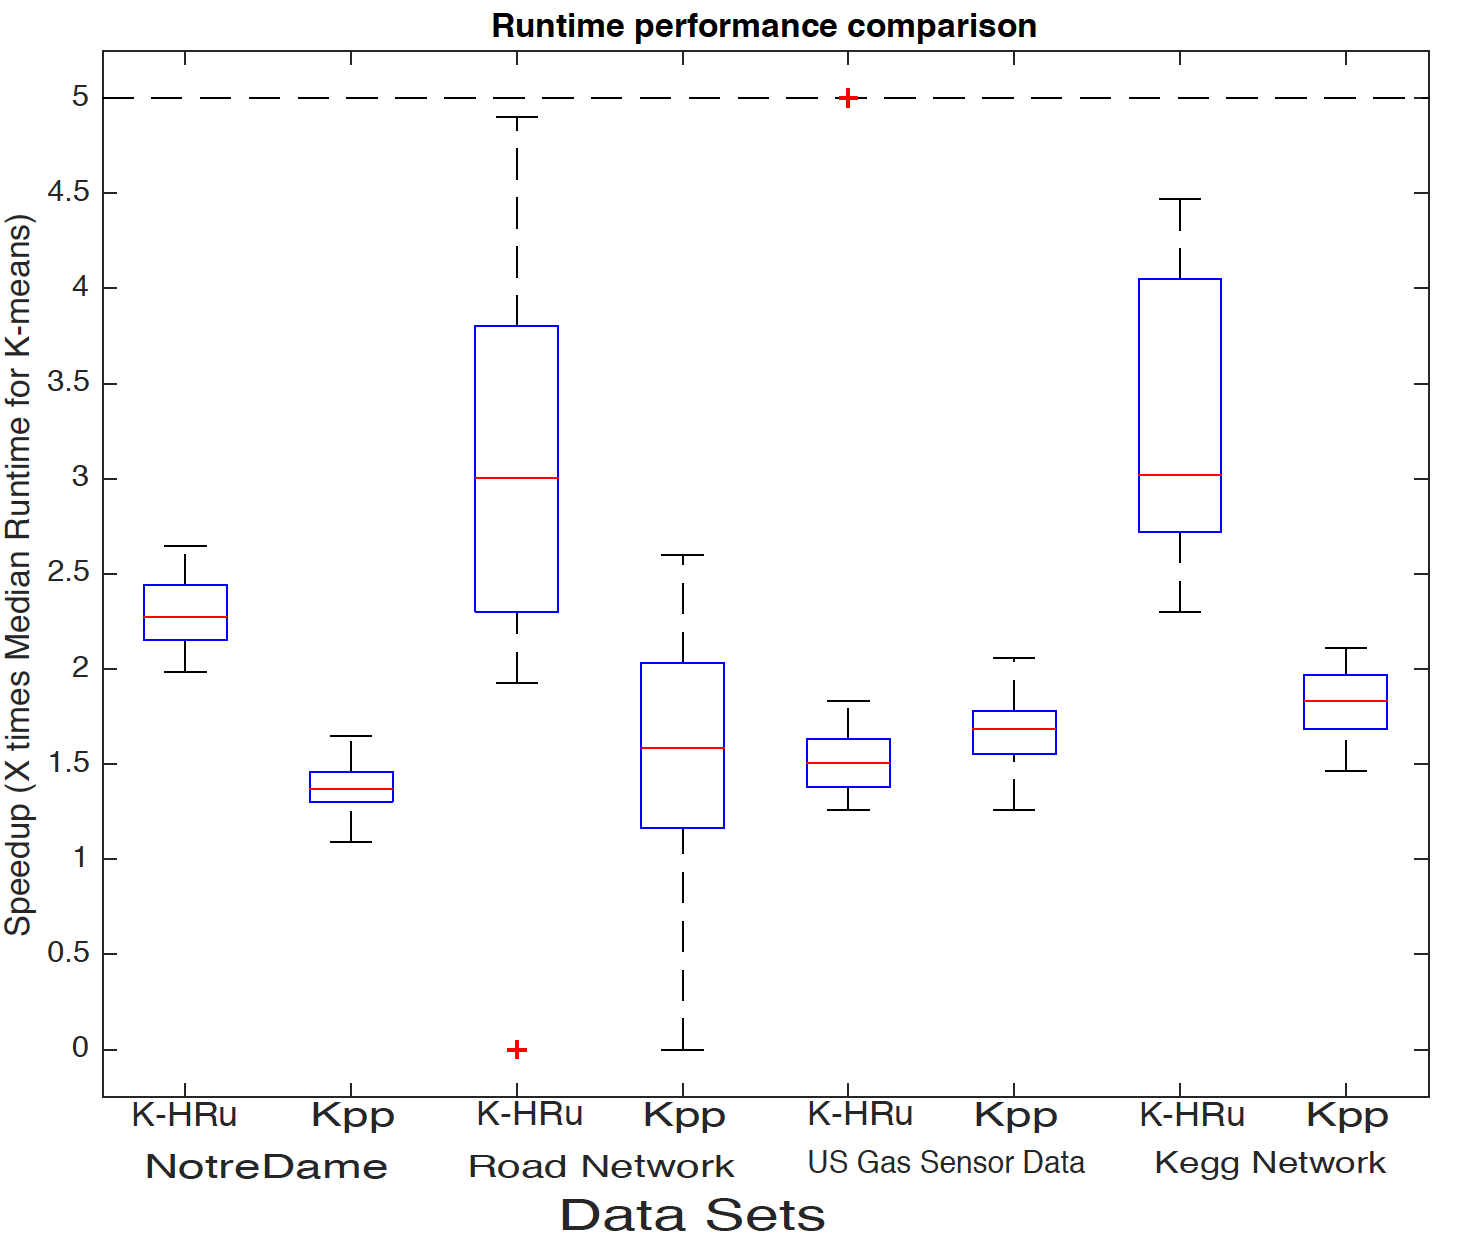
\includegraphics[width=\textwidth,  height=7cm,keepaspectratio]{kpp+k_cust_speedup_small}
    \caption{Median Speed up, Small Data (k=240)(*K-HRu: K-Means-History Reuse; Kpp: K-Means++)}
    \centering
    \label{fig:box_speedup_small}
\end{figure}

\begin{figure}[b!]
    \centering
    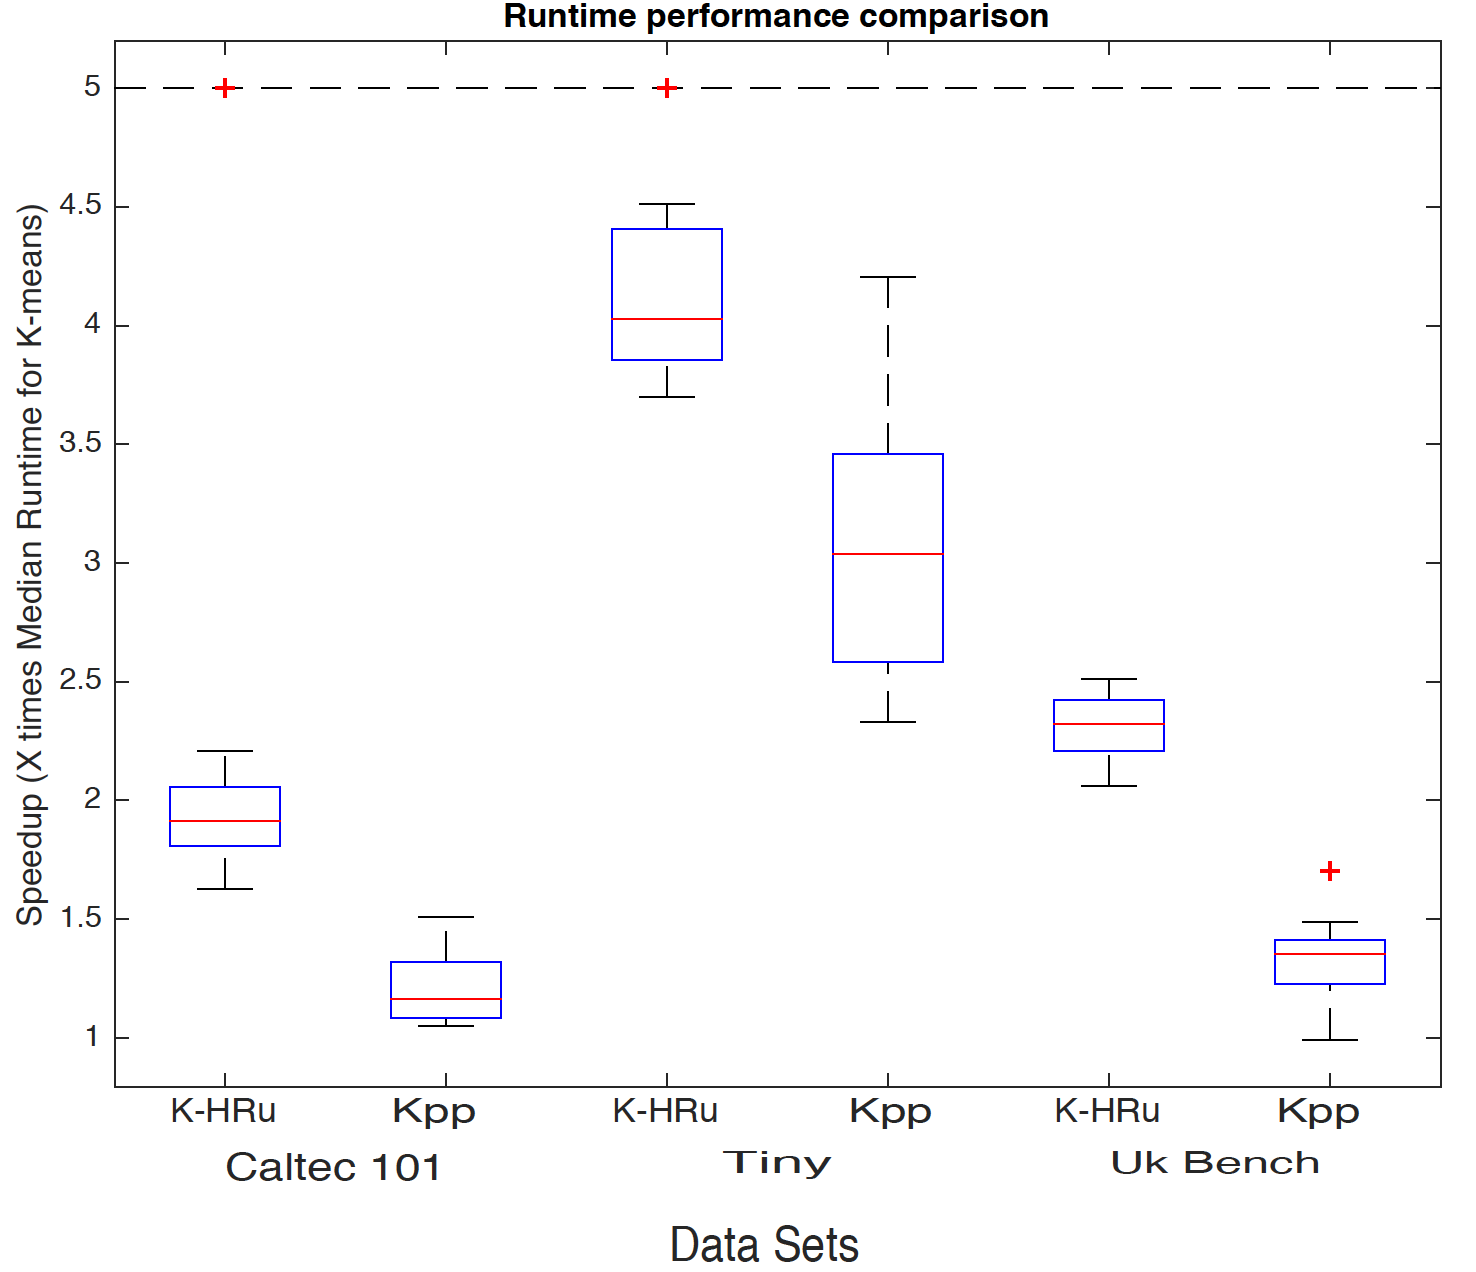
\includegraphics[width=\textwidth , height=7cm,keepaspectratio]{kcust+kpp_speedup_large}
    \caption{Median Speed up, Large Data (k=600)(*K-HRu: K-Means-History Reuse; Kpp: K-Means++)}
    \label{fig:box_speedup_large}
\end{figure}

Another interesting feature seen in the above box plots is the varying degrees of speed up seen for the various segments for same data sets. Looking at the speed up that \textit{K-Means with History Reuse} achieves over the original \textit{K-Means (Lloyd’s algorithm)} we can see that the speed up is generally spread out over a larger range as compared to the performance of the \textit{K-Means++ algorithm} as compared to \textit{Lloyd’s Algorithm}. This thus, brings to fore our above made assumption about the quality of history data set available in terms of the probability of similarity . Our experiments prove our intuitive hypothesis that probabilistically similar data sets will tend to be classed together into similar clusters, thus making them the best history match data sets. The larger variance seen in the box plots above is testament to this. Normalization using \textit{PCA} of data sets, tends to mitigate this to a large extent thus providing us the ability to use history data not along same planes as well and thus providing a consistent speed up, but a better match of normalized data would provide even higher speed ups. We consistently saw that maximum speed ups are seen when the probability of similarity is higher. For segment with high probabilistic similarity we saw speed ups of up to and above \textit{\textbf{100 X}}.

\section{Future Work}
\label{chap-six}
As we have seen in our experimentation the speedup in the run time for the algorithm is dependent of the quality (probability of similarity) of historically available data sets for selection. Better quality selection would lead to better speedups. Thus one future work could involve new methodology for maintaining best quality history data sets.
Another possibility is to explore this History Reuse methodology for other algorithms. The general use of determining best match history data set is generic in nature (i.e. independent of the K-Means algorithm in itself) and thus can be extended to other algorithms such as the \textit{SVD based SVM algorithm}. Only a minor change to the training step specific to K-Means is required in such a case. This thus can be used to prove the comprehensible usability of this algorithm for all algorithms in the same class.
On the systems side the History reuse methodology can be used for memory data validation in Non Volatile Memory (NVM). This would prevent multiple expensive re-writes to NVM from main memory in case of already existing data.

Another area to explore may be the use of non uniform generation of hostogram for a better sample size selection in case of the screening algorithm. We chose not to explore this avenue in current work because our technique for unform buckets was showing significant performance gains. \cite{non_uniform_hist_1} shows an interesting way for generating non uniform histograms while still capturing sufficient desnity information such as to facilitate the selection of the density information more succinctly. Integral Histogram\cite{non_uniform_hist_2} represent a new a way of capturing non uniform histograms in the cartesian space and my be extended to our use as well. Both these above mentioned methods may help with furhter improving the accuracy of the screening algorithm.

\section{Conclusion}
\label{chap-seven}
In conclusion we would like to say that probabilistic metric for data-set comparison is
one of the best metrics for this purpose. It tells us the exact degree to which we can
expect the computation reuse to be successful for any historical data-set. It also represents a generic way of ranking data sets based on similarity and may have many more applications than just in history-reuse computation. We have also seen based on the above
results that the above mentioned algorithm is handy for all data sets irrespective if the dimensionality, cardinality or cluster count for the data set.
Though the algorithm shows speedups for all data sets for all cluster indexes we see a substantially higher speedup for larger cluster counts as this results in a speedup in both, the run time of the algorithm as well as the initialization step for the algorithm. The initialization is sped up considerably by our approach and this plays a vital part in the final speedup for larger cluster counts as intialization becomes a significant amount of the run time for both the \textit{Random K-Means} and the \textit{K-Means++} algorithm.
Since this can be used as a drop in replacement for any initialization method, it can be used with any flavour of the original K-Means Algorithm.t preserves the semantic of the original K-means. These appealing properties, plus its simplicity, make it a
practical replacement of the standard K-means as long as viable historical data sets are available for reuse.

\balance


% \section{References}
% \begin{itemize}
%     \item OpenCV: docs.opencv.org/
%     \item T-Test:
%     \begin{itemize}
%         \item https://en.wikipedia.org/wiki/Student%27s_t-test
%     \end{itemize} 
%     \item: K-Means: https://en.wikipedia.org/wiki/K-Means%2B%2B
%     \item: K-Means++: http://www.cse.buffalo.edu/faculty/miller/Courses/CSE633/Chandramohan-Fall-2012-CSE633.pdf
%     \item  Python References:
%     \begin{itemize}
%         \item https://docs.python.org/2/extending/extending.html
%     \end{itemize}
%     \item C++ Documentations: http://www.cplusplus.com/doc/
%     \item Community help (OpenCV)
%     \begin{itemize}
%         \item http://answers.opencv.org/questions/
%     \end{itemize}
%     \item Community help (Python-C++Interface):
%     \begin{itemize}
%         \item http://stackoverflow.com/questions/30089716/pythoc-funtion-call-from-cpp
%     \end{itemize}
%     \item Community help (T-Test):
%     \begin{itemize}
%         \item http://stackoverflow.com/questions/30023032/pca-computation-using-opencv-use-return-value
%         \item http://stackoverflow.com/questions/30090926/python-runtime-error-on-running-t-test
%     \end{itemize}
% \end{itemize}

% \appendix
% %Appendix A
% \section{Headings in Appendices}
% \subsection{Introduction}
% \subsection{Motivation}
% \subsection{Objectives}
% \subsection{Framework}
% \subsubsection{Feature Set Reduction}
% \subsubsection{Similarity Metric Calculation}
% \subsubsection{History Storage Architecture}
% \subsubsection{Matcher and Selector}
% \subsection{Challenges}
% \subsubsection{Reducing Data-set dimension size:}
% \subsubsection{Reducing Data-points:}
% \subsubsection{Other Challenges:}
% \subsection{Results}
% \subsection{Remaining Issues and Possible solutions}
% \subsection{Lessons and Experiences}
% \subsection{Conclusion}
% \subsection{Acknowledgement}
% \subsection{References}
% \end{appendix}

\medskip

% \printbibliography{blah.bib}
% \bibliographystyle{abbrv}
% \bibliography{blah.bib}
% \bibliographystyle{abbrv}
% \bibliography{sample}

% The following two commands are all you need in the
% initial runs of your .tex file to
% produce the bibliography for the citations in your paper.
\bibliographystyle{abbrv}
\bibliography{vldb_sample}  % vldb_sample.bib is the name of the Bibliography in this case
% You must have a proper ".bib" file
%  and remember to run:
% latex bibtex latex latex
% to resolve all references



\end{document}
